\documentclass[11pt]{article}

\usepackage[margin=1in]{geometry}
\usepackage{microtype}
\usepackage{amsmath,amssymb,amsthm,mathtools}
\usepackage{mathrsfs}
\usepackage{bm}
\usepackage{booktabs}
\usepackage{array}
\usepackage{enumitem}
\usepackage{xcolor}
\usepackage{tikz}
\usepackage{pgfplots}
\usepackage{hyperref}
\usepackage[nameinlink,capitalise,noabbrev]{cleveref}

\pgfplotsset{compat=1.18}
\usetikzlibrary{arrows.meta,positioning,calc,decorations.pathreplacing}

\hypersetup{
  colorlinks=true,
  linkcolor=blue!55!black,
  citecolor=blue!55!black,
  urlcolor=blue!55!black,
  pdftitle={Square-Prefix Smooth--Transport Matching in Squared Complex Factor Space},
  pdfauthor={Fred Viole}
}

\setlength{\parindent}{0pt}
\setlength{\parskip}{0.55em}
\allowdisplaybreaks

\definecolor{ovvoblue}{RGB}{31,78,121}
\definecolor{ovvogreen}{RGB}{37,116,84}
\definecolor{ovvored}{RGB}{162,55,55}
\definecolor{ovvogray}{RGB}{88,96,105}

\newtheorem{theorem}{Theorem}[section]
\newtheorem{proposition}[theorem]{Proposition}
\newtheorem{lemma}[theorem]{Lemma}
\newtheorem{corollary}[theorem]{Corollary}
\newtheorem{conjecture}[theorem]{Conjecture}
\theoremstyle{definition}
\newtheorem{definition}[theorem]{Definition}
\newtheorem{example}[theorem]{Example}
\theoremstyle{remark}
\newtheorem{remark}[theorem]{Remark}
\newtheorem{caution}[theorem]{Caution}
\crefname{conjecture}{conjecture}{conjectures}
\Crefname{conjecture}{Conjecture}{Conjectures}

\newcommand{\eps}{\varepsilon}
\newcommand{\Pplus}{P^{+}}
\newcommand{\1}{\mathbf{1}}
\newcommand{\vect}[1]{\bm{#1}}
\newcommand{\ip}[2]{\left\langle #1,#2\right\rangle}
\newcommand{\norm}[1]{\left\lVert #1\right\rVert}
\newcommand{\R}{\mathbb{R}}
\newcommand{\N}{\mathbb{N}}
\newcommand{\Z}{\mathbb{Z}}
\newcommand{\C}{\mathbb{C}}
\newcommand{\Repart}{\operatorname{Re}}
\newcommand{\Impart}{\operatorname{Im}}
\newcommand{\card}{\operatorname{card}}

\title{\textbf{Square-Prefix Smooth--Transport Matching\\
in Squared Complex Factor Space}\\[0.45em]
\large Canonical cofactor parabolas, a moving cutoff,\\
and the $2ab$ lifetime--clustering mechanism}
\author{Fred Viole\\OVVO Labs}
\date{July 2026}

\begin{document}
\maketitle

\begin{abstract}
Let
\[
 B_n=[n^2,(n+1)^2),\qquad
 R_n=n+1,\qquad
 X_n=R_n^2-1,
\]
and define the complete square-prefix Mertens value
\[
 S_n=M(X_n)=\sum_{m\le X_n}\mu(m).
\]
At the exact square-root cutoff, every squarefree $m\le X_n$ is uniquely either $R_n$-smooth or of the form $cq$ with $c<R_n<q$ and $q$ prime.  This gives the unconditional identity
\[
 S_n=A_n-T_n.
\]

The factor geometry is placed entirely in the squared complex plane.  For a factor pair $cq=m$, define
\[
 a=\frac{c+q}{2},\qquad b=\frac{q-c}{2},
\]
with signed $b$, and square
\[
 w=(a+bi)^2=m+iY,
 \qquad
 Y=2ab=\frac{q^2-c^2}{2}.
\]
Writing $w=x+iy$ and $\rho=|w|$, the factors are recovered exactly by
\[
 c^2=\rho-y,\qquad q^2=\rho+y.
\]
Thus the squared point carries the source integer, the cofactor, the largest prime, the factor imbalance, the prefix-entry time, and the smoothness-transition time.

The paper distinguishes the \emph{full factor fibre} of a fixed integer from the \emph{canonical M\"obius point} used by the smooth--transport decomposition.  The full fibre contains every factor pair and has the universal odd-factor envelope
\[
 0\le Y\le\frac{N^2-1}{2};
\]
the familiar bound with smallest factor $3$ is the nontrivial odd-factor envelope
\[
 Y\le\frac{N^2-81}{18}.
\]
The canonical point instead uses
\[
 q=\Pplus(m),\qquad c=m/q,
\]
so $b$ and $Y$ may be negative when the remaining cofactor exceeds the largest prime.

For fixed cofactor $c$, the canonical points lie on the parabola
\[
 \gamma_c(x)=\frac{x^2-c^4}{2c^2},
\]
subject to the exact arithmetic conditions that $c$ is squarefree and $q=x/c$ is prime with $q>\Pplus(c)$.  At cutoff $R$, the complete prefix is the vertical strip $x<R^2$, while the smooth--transport boundary is the moving parabola
\[
 \Gamma_R(x)=\frac{R^4-x^2}{2R^2}.
\]
The two parabolas meet exactly at
\[
 \gamma_c(x)=\Gamma_R(x)\iff x=cR,
\]
and they meet orthogonally.  Since an actual point on $\gamma_c$ has $x=cq$, the intersection is precisely the transition $q=R$.

This yields an exact moving-region interpretation of $A_n-T_n$.  A point enters the prefix when the vertical boundary reaches $x=m$, occupies the transport region while $\sqrt m<R<q$, and then crosses into the smooth region at $R=q$.  The crossing mass appears with opposite signs in the increments of $A$ and $-T$ and therefore telescopes identically.  Only new points entering through the square-block strip contribute to the residual increment.

The same ordinate $Y=2ab$ controls both spatial clustering and temporal persistence.  For a canonical point in $B_n$, if $|Y|\le H$, then the factor gap $|q-c|$ is at most $H/n$, and for each fixed gap there is at most one product in $B_n$.  Hence
\[
 \#\{m\in B_n:|Y_m|\le H\}
 \le \left\lfloor\frac{H}{n}\right\rfloor,
\]
with no points at all for $|Y_m|\le n$.
For transport points,
\[
 L(m)\le q-\sqrt{cq}
 =\frac{2Y}{q(1+\sqrt{c/q})(1+c/q)}
 \le\frac{2Y}{q}.
\]
At the natural height $H\asymp n$, both block occupancy and transport lifetime are $O(1)$.

Finally, the quadratic map
\[
 \Phi(c,q)=\left(cq,\frac{q^2-c^2}{2}\right)
\]
is conformal: its differential expands both coordinate directions by $\sqrt{c^2+q^2}$ and its Jacobian is
\[
 \det D\Phi=c^2+q^2\ge2cq.
\]
At square scale $cq\asymp n^2$, unit factor-lattice area expands by at least order $n^2$, exactly the two-power dilution required to pass from the coherent $N^5$ ceiling to the cubic $N^3$ scale.  Turning this geometric dilution into a signed high-shell kernel estimate is the remaining analytic step.  The arithmetic decomposition, all coordinate identities, the moving-region partition, the channel telescoping law, the conformal Jacobian, and the low-height clustering and lifetime bounds are unconditional.
\end{abstract}

\tableofcontents
\newpage

%======================================================================
\section{Introduction and principal results}
\label{sec:introduction}
%======================================================================

The square-prefix framework organizes the Mertens function at the complete boundaries
\[
 X_n=(n+1)^2-1.
\]
Its arithmetic advantage is that the cutoff has an exact square root.  A squarefree integer below $R^2$ cannot contain two prime factors larger than $R$.  Consequently, every nonsmooth source has a unique largest-prime representation $m=cq$ with
\[
 c<R<q.
\]
This produces the exact decomposition
\[
 S_n=A_n-T_n.
\]

The geometric question is why the two large components $A_n$ and $T_n$ match closely enough that their residual remains on the conjectural cubic energy scale.  The answer developed here uses the squared complex factor coordinate
\[
 (a+bi)^2=m+2abi.
\]
The key observation is not merely that the factor hyperbola becomes a vertical line.  The entire smooth--transport process becomes a moving partition of a fixed signed point cloud:

\begin{enumerate}[leftmargin=1.7em,itemsep=0.35em]
\item each squarefree source has one canonical point in the squared complex plane;
\item fixed cofactors generate explicit parabolic curves;
\item the prefix cutoff is a moving vertical line;
\item the smoothness cutoff is a moving parabola;
\item every canonical point follows the state path
\[
 \text{outside}\longrightarrow\text{transport}\longrightarrow\text{smooth};
\]
\item the transport-to-smooth crossing telescopes exactly;
\item the vertical coordinate $2ab$ measures both factor separation and transport lifetime;
\item the quadratic map expands factor-lattice area by $c^2+q^2\asymp n^2$ at square scale $n$.
\end{enumerate}

The main exact results are summarized below.

\begin{theorem}[Exact square-root decomposition]
\label{thm:intro-decomposition}
For $R_n=n+1$ and $X_n=R_n^2-1$, define
\begin{align*}
 A_n&:=\sum_{\substack{m\le X_n\\\Pplus(m)\le R_n}}\mu(m),\\
 T_n&:=\sum_{c<R_n}\mu(c)
 \left[
 \pi\!\left(\left\lfloor\frac{X_n}{c}\right\rfloor\right)-\pi(R_n)
 \right].
\end{align*}
Then
\[
 \boxed{S_n=A_n-T_n.}
\]
\end{theorem}

\begin{theorem}[Squared-space recovery]
\label{thm:intro-recovery}
Let $w=x+iy$ be generated by a positive factor pair $cq=x$ through
\[
 y=\frac{q^2-c^2}{2}.
\]
With $\rho=|w|$,
\[
 \boxed{c^2=\rho-y,\qquad q^2=\rho+y.}
\]
Hence the squared point determines the ordered factor pair exactly.
\end{theorem}

\begin{theorem}[Cofactor-curve cutoff intersection]
\label{thm:intro-intersection}
For fixed $c>0$, put
\[
 \gamma_c(x)=\frac{x^2-c^4}{2c^2}.
\]
At cutoff $R>0$, put
\[
 \Gamma_R(x)=\frac{R^4-x^2}{2R^2}.
\]
Then
\[
 \boxed{\gamma_c(x)=\Gamma_R(x)\iff x=cR.}
\]
The curves meet orthogonally at their intersection.  At an arithmetic point $x=cq$, the sign of $\gamma_c(cq)-\Gamma_R(cq)$ is the sign of $q-R$.
\end{theorem}

\begin{theorem}[Exact channel telescoping]
\label{thm:intro-telescoping}
As $R$ increases, a canonical point enters the prefix at $R=\sqrt{cq}$ and crosses from transport to smooth at $R=q$.  The signed mass crossing the moving parabola appears with opposite signs in the increments of $A$ and $-T$.  Therefore all internal channel transfers cancel from the increment of $A-T$; only points entering the new square strip remain.
\end{theorem}

\begin{theorem}[Low-height clustering and lifetime]
\label{thm:intro-low}
Let $m=cq\in B_n$ be canonical and let
\[
 Y_m=\frac{q^2-c^2}{2}.
\]
Then, for $H\ge0$,
\[
 \#\{m\in B_n:|Y_m|\le H\}
 \le\left\lfloor\frac{H}{n}\right\rfloor,
\]
and the count is zero when $H=n$.  For odd sources the bound improves to
$\lfloor H/(2n)\rfloor$.
If $Y_m>0$, the transport lifetime satisfies
\[
 L(m)\le\frac{2Y_m}{q}.
\]
Consequently, for fixed $\Lambda$, the canonical points with $|Y_m|\le\Lambda n$ have uniformly bounded block occupancy, and the transport members have uniformly bounded lifetime.
\end{theorem}

\begin{theorem}[Major-arc rank-one law for cofactor blocks]
\label{thm:intro-major-rank-one}
Fix $\eta>0$ and a dyadic cofactor scale $C\asymp N^\alpha$ with
$0\le\alpha\le1-\eta$.  On the local square-prefix interval
$N\le n<2N$, let
\[
 B_C(n):=-\sum_{C<c\le2C}\mu(c)\Pi_c(X_n),
 \qquad
 a_C:=\sum_{C<c\le2C}\frac{\mu(c)}{c},
\]
and let $P_n=-\pi(X_n)$ be the prime-curve vector.  Then
\[
 \boxed{
 B_C(n)=\frac{2}{2-\alpha}\,a_C P_n
 +O_\eta\!\left(\frac{N^2}{\log^2N}\right)
 }
\]
uniformly for $N\le n<2N$.  Consequently, the local Gram matrix of any
fixed collection of such cofactor blocks is a rank-one prime-curve main
term plus an error of order $O_\eta(N^5/\log^3N)$ entrywise.
\end{theorem}

\begin{theorem}[Quadratic conformal expansion]
\label{thm:intro-jacobian}
The map
\[
 \Phi(c,q)=\left(cq,\frac{q^2-c^2}{2}\right)
\]
has
\[
 D\Phi(c,q)^{\mathsf T}D\Phi(c,q)
 =(c^2+q^2)I,
\]
and
\[
 \det D\Phi(c,q)=c^2+q^2\ge2cq.
\]
At square scale $cq\asymp n^2$, lengths expand by at least order $n$ and areas by at least order $n^2$.
\end{theorem}

The remaining theorem is an operator estimate: prove that the high-height, cross-curve signed interactions inherit this geometric dilution when inserted into the exact square-prefix kernel.  No claim is made that a coordinate change alone proves cancellation; the point is that the coordinate change exposes the exact two-power scale and localizes the unresolved interaction.

%======================================================================
\section{Square prefixes and the exact arithmetic split}
\label{sec:arithmetic}
%======================================================================

Define the complete square block
\begin{equation}
 B_n:=\{m\in\N:n^2\le m<(n+1)^2\},
 \label{eq:block}
\end{equation}
the square-root cutoff
\begin{equation}
 R_n:=n+1,
 \label{eq:Rn}
\end{equation}
and the complete-prefix endpoint
\begin{equation}
 X_n:=R_n^2-1=(n+1)^2-1.
 \label{eq:Xn}
\end{equation}
The square-prefix Mertens value is
\begin{equation}
 S_n:=M(X_n)=\sum_{m\le X_n}\mu(m).
 \label{eq:Sn}
\end{equation}
Because $\mu(R_n^2)=0$ for $R_n>1$, one may equally write $S_n=M(R_n^2)$.

Write $\Pplus(m)$ for the largest prime factor of $m$, with $\Pplus(1)=1$.

\begin{definition}[Smooth and transport terms]
\label{def:AT}
Define
\begin{align}
 A_n
 &:={\sum}_{\substack{1\le m\le X_n\\\Pplus(m)\le R_n}}\mu(m),
 \label{eq:An}\\
 T_n
 &:={\sum}_{1\le c<R_n}\mu(c)
 \left[
 \pi\!\left(\left\lfloor\frac{X_n}{c}\right\rfloor\right)-\pi(R_n)
 \right].
 \label{eq:Tn}
\end{align}
\end{definition}

\begin{lemma}[One-large-prime closure]
\label{lem:one-large}
Let $m\le R^2-1$ be squarefree.  If $\Pplus(m)>R$, then there is a unique factorization
\begin{equation}
 m=cq,
 \qquad
 1\le c<R<q,
 \qquad
 q\text{ prime},
 \label{eq:one-large}
\end{equation}
where $q=\Pplus(m)$.  Moreover,
\begin{equation}
 \mu(m)=-\mu(c).
 \label{eq:mobius-peel}
\end{equation}
\end{lemma}

\begin{proof}
Put $q=\Pplus(m)$ and $c=m/q$.  If $c\ge R$, then $m=cq>R^2$, contrary to $m\le R^2-1$.  Since $m$ is squarefree, $q\nmid c$ and $\mu(cq)=-\mu(c)$.  Uniqueness follows from the largest-prime choice.
\end{proof}

\begin{proof}[Proof of \cref{thm:intro-decomposition}]
Partition the squarefree $m\le X_n$ according to whether $\Pplus(m)\le R_n$ or $\Pplus(m)>R_n$.  The first population contributes $A_n$.  By \cref{lem:one-large}, the second population is uniquely $m=cq$ with $c<R_n<q$, and each source has weight $-\mu(c)$.  The total second contribution is therefore $-T_n$.
\end{proof}


\subsection{The exact largest-prime cofactor identity}
\label{subsec:central-identity}

For $c\ge1$, define the prime-tail counting function
\begin{equation}
 \Pi_c(x)
 :=
 \#\left\{
 q\text{ prime}:
 \Pplus(c)<q\le\left\lfloor\frac{x}{c}\right\rfloor
 \right\}.
 \label{eq:Pi-c}
\end{equation}
Equivalently,
\begin{equation}
 \Pi_c(x)
 =
 \left(
 \pi\!\left(\left\lfloor\frac{x}{c}\right\rfloor\right)
 -\pi(\Pplus(c))
 \right)_{+},
 \label{eq:Pi-c-positive-part}
\end{equation}
where $(u)_+:=\max\{u,0\}$.  The positive part is essential when
$x/c<\Pplus(c)$.

\begin{theorem}[Exact largest-prime cofactor expansion]
\label{thm:central-M-identity}
For every real $x\ge1$,
\begin{equation}
 \boxed{
 M(x)
 =
 1-\sum_{c\ge1}\mu(c)\Pi_c(x).
 }
 \label{eq:central-M-identity-compact}
\end{equation}
The sum is finite, and separating the prime curve $c=1$ gives
\begin{equation}
 \boxed{
 M(x)
 =
 1-\pi(x)
 -\sum_{2\le c\le x/2}
 \mu(c)
 \left(
 \pi\!\left(\left\lfloor\frac{x}{c}\right\rfloor\right)
 -\pi(\Pplus(c))
 \right)_{+}.
 }
 \label{eq:central-M-identity}
\end{equation}
\end{theorem}

\begin{proof}
Every squarefree $m>1$ has a unique largest prime factor
$q=\Pplus(m)$.  Writing $c=m/q$, one has
\[
 q>\Pplus(c),
 \qquad
 \mu(m)=\mu(cq)=-\mu(c).
\]
Conversely, every pair consisting of a squarefree $c$ and a prime
$q>\Pplus(c)$ produces the squarefree integer $m=cq$ whose largest
prime factor is $q$.  The condition $m\le x$ is exactly $q\le x/c$.
Summing $-\mu(c)$ over these unique pairs proves
\cref{eq:central-M-identity-compact}.  The $c=1$ term is
$-\pi(x)$, because $\Pplus(1)=1$.  No term with $c>x/2$ can occur.
\end{proof}

\begin{remark}[Central analytic engine]
\Cref{eq:central-M-identity} is the exact arithmetic form of the
cofactor-parabola decomposition.  It shows that the Mertens function is
not obtained by proving that the prime curve is small.  The prime curve
$-\pi(x)$ is cancelled by the M\"obius-weighted collection of all
curves $c\ge2$.  The geometric and large-sieve parts of the paper are
methods for controlling the rate of this exact cancellation on square
prefixes.
\end{remark}


\subsection{An unconditional major-arc rank-one theorem}
\label{subsec:major-rank-one}

The first analytic component of the cofactor cascade can be proved
unconditionally.  It explains why the small-cofactor Gram matrix is
nearly rank one and identifies the scalar coefficients governing its
large coherent mode.

For a dyadic block $C<c\le2C$, define
\begin{equation}
 B_C(n)
 :=-\sum_{C<c\le2C}\mu(c)\Pi_c(X_n),
 \qquad
 a_C:=\sum_{C<c\le2C}\frac{\mu(c)}{c},
 \label{eq:block-vector-aC}
\end{equation}
and write
\begin{equation}
 P_n:=-\pi(X_n).
 \label{eq:prime-vector-P}
\end{equation}

\begin{theorem}[Polynomial-range major-arc rank-one law]
\label{thm:major-rank-one}
Fix $\eta>0$.  Let $N$ tend to infinity, let
$0\le\alpha\le1-\eta$, and choose a dyadic $C$ satisfying
$C\asymp N^\alpha$.  Uniformly for $N\le n<2N$,
\begin{equation}
 \boxed{
 B_C(n)
 =\lambda_\alpha a_C P_n
 +O_\eta\!\left(\frac{N^2}{\log^2N}\right),
 \qquad
 \lambda_\alpha:=\frac{2}{2-\alpha}.
 }
 \label{eq:major-rank-one-pointwise}
\end{equation}
Consequently,
\begin{equation}
 \sum_{N\le n<2N}
 \left|B_C(n)-\lambda_\alpha a_C P_n\right|^2
 \ll_\eta \frac{N^5}{\log^4N}.
 \label{eq:major-rank-one-L2}
\end{equation}
If $D\asymp N^\beta$ with $0\le\beta\le1-\eta$, then
\begin{equation}
 \boxed{
 \langle B_C,B_D\rangle_{[N,2N)}
 =\lambda_\alpha\lambda_\beta a_Ca_D
 \|P\|_{[N,2N)}^2
 +O_\eta\!\left(\frac{N^5}{\log^3N}\right).
 }
 \label{eq:major-rank-one-Gram}
\end{equation}
\end{theorem}

\begin{proof}
For $c\asymp N^\alpha$ and $N\le n<2N$, one has
$X_n/c\gg_\eta N^{1+\eta}$, while $\Pplus(c)\le c\ll N^{1-\eta}$.
Thus, for sufficiently large $N$, the positive part in $\Pi_c(X_n)$ is
inactive and
\[
 \Pi_c(X_n)=\pi(X_n/c)-\pi(\Pplus(c)).
\]
The prime number theorem with its standard first remainder term gives,
uniformly in this range,
\[
 \pi(X_n/c)
 =\frac{X_n/c}{\log(X_n/c)}
 +O_\eta\!\left(\frac{X_n}{c\log^2N}\right),
\]
and
\[
 \pi(X_n)
 =\frac{X_n}{\log X_n}
 +O\!\left(\frac{X_n}{\log^2N}\right).
\]
Since
\[
 \frac{\log X_n}{\log(X_n/c)}
 =\frac{2}{2-\alpha}+O_\eta\!\left(\frac1{\log N}\right),
\]
it follows that
\[
 \pi(X_n/c)
 =\frac{\lambda_\alpha}{c}\pi(X_n)
 +O_\eta\!\left(\frac{N^2}{c\log^2N}\right).
\]
Summing the error uses
$\sum_{C<c\le2C}c^{-1}\ll1$.  The fixed lower-prime exclusions satisfy
\[
 \sum_{C<c\le2C}\pi(\Pplus(c))
 \le\sum_{C<c\le2C}c
 \ll C^2
 \ll_\eta N^{2-2\eta},
\]
which is absorbed by $N^2/\log^2N$.  This proves
\cref{eq:major-rank-one-pointwise}.  Squaring and summing over $N$ local
prefixes gives \cref{eq:major-rank-one-L2}.  Finally, write each block as
its prime-vector main term plus its error and apply Cauchy--Schwarz,
using $\|P\|_{[N,2N)}\asymp N^{5/2}/\log N$.
\end{proof}

\begin{corollary}[Rank-one major-arc Gram matrix]
\label{cor:rank-one-Gram}
For finitely many polynomial cofactor blocks with exponents bounded by
$1-\eta$, their local Gram matrix has the form
\begin{equation}
 G_N
 =\|P\|_{[N,2N)}^2\,vv^{\mathsf T}+E_N,
 \qquad
 v_j=\lambda_{\alpha_j}a_{C_j},
 \label{eq:Gram-rank-one-form}
\end{equation}
with every entry of $E_N$ bounded by
$O_\eta(N^5/\log^3N)$.  Thus the coherent major-arc component cancels
between dyadic cofactor blocks entirely through the scalar harmonic
M\"obius coefficients $a_{C_j}$, before any minor-arc estimate is used.
\end{corollary}

\begin{remark}[What this theorem accomplishes]
\Cref{thm:major-rank-one} is a genuine major-arc cancellation theorem
for substantial ranges $C\asymp N^\alpha$, $\alpha<1$.  It is not RH:
it does not control cofactor scales $C\gtrsim N$, nor does it supply a
power saving for the rank-one remainder.  It does prove that the large
small-cofactor interactions are analytically organized rather than
arbitrary, and it identifies the exact main term that the
Squared-Cofactor Large Sieve must remove.
\end{remark}

For
\[
 \vect A_N=(A_1,\ldots,A_N)^{\mathsf T},
 \quad
 \vect T_N=(T_1,\ldots,T_N)^{\mathsf T},
 \quad
 \vect S_N=(S_1,\ldots,S_N)^{\mathsf T},
\]
we have
\begin{equation}
 \vect S_N=\vect A_N-\vect T_N
 \label{eq:vector-AT}
\end{equation}
and
\begin{equation}
 \sum_{n\le N}|S_n|^2
 =\norm{\vect A_N-\vect T_N}_2^2.
 \label{eq:energy-AT}
\end{equation}

%======================================================================
\section{The full factor fibre of a fixed integer}
\label{sec:full-fibre}
%======================================================================

The factorization geometry and the smooth--transport geometry use the same coordinate map but different point selections.  This distinction is essential.

Fix $N\ge1$ and consider every positive factor pair
\begin{equation}
 uv=N,
 \qquad
 1\le u\le v.
 \label{eq:factor-pair}
\end{equation}
Define the Fermat coordinates
\begin{equation}
 a=\frac{u+v}{2},
 \qquad
 b=\frac{v-u}{2}\ge0.
 \label{eq:full-Fermat}
\end{equation}
Then
\begin{equation}
 u=a-b,
 \qquad
 v=a+b,
 \qquad
 N=a^2-b^2.
 \label{eq:full-recovery}
\end{equation}
The coordinates lie in $\frac12\Z$; they are integers when $u$ and $v$ have the same parity.

Squaring the complex factor gives
\begin{equation}
 (a+bi)^2=N+iY,
 \qquad
 \boxed{Y=2ab=\frac{v^2-u^2}{2}.}
 \label{eq:full-square}
\end{equation}
Thus all factorizations of a fixed $N$ lie on the vertical fibre
\begin{equation}
 \Repart w=N.
 \label{eq:vertical-fibre}
\end{equation}

\subsection{Exact square-root tests}

Let
\begin{equation}
 w=N+iY,
 \qquad
 \rho=|w|=\sqrt{N^2+Y^2}.
 \label{eq:rho-full}
\end{equation}
Then
\begin{align}
 a^2&=\frac{\rho+N}{2},
 \label{eq:a-square}\\
 b^2&=\frac{\rho-N}{2},
 \label{eq:b-square}\\
 u^2&=\rho-Y,
 \label{eq:u-square}\\
 v^2&=\rho+Y.
 \label{eq:v-square}
\end{align}
Accordingly, a candidate vertical ordinate $Y$ corresponds to an exact factorization if and only if the relevant square and parity conditions hold.  The identity
\begin{equation}
 \sqrt{N^2+Y^2}=a^2+b^2
 \label{eq:hypotenuse}
\end{equation}
is the right-triangle form of the same condition.

\subsection{The full admissible intervals}

For a factor pair $u(N/u)=N$ with $1\le u\le\sqrt N$,
\begin{equation}
 a(u)=\frac{u+N/u}{2},
 \qquad
 b(u)=\frac{N/u-u}{2}.
 \label{eq:ab-u}
\end{equation}
Both functions decrease as $u$ increases toward $\sqrt N$.  Therefore the full positive factor fibre satisfies
\begin{align}
 \sqrt N&\le a\le\frac{N+1}{2},
 \label{eq:a-full-range}\\
 0&\le b\le\frac{N-1}{2},
 \label{eq:b-full-range}\\
 0&\le Y\le\frac{N^2-1}{2}.
 \label{eq:Y-full-range}
\end{align}
For integer enumeration one uses $a\ge\lceil\sqrt N\rceil$ with the parity required by $N$.

The upper endpoint corresponds to the trivial factor pair $1\cdot N$.  If the trivial factor is excluded and the smallest permitted odd factor is $3$, then
\begin{align}
 a&\le\frac{N+9}{6},
 \label{eq:a-three}\\
 b&\le\frac{N-9}{6},
 \label{eq:b-three}\\
 Y&\le\frac{N^2-81}{18}.
 \label{eq:Y-three}
\end{align}
These are the nontrivial odd-factor or semiprime-search envelopes.  They are not the universal bounds for the complete factor fibre.

\begin{example}[The fibre $N=309$]
The trivial factor pair $1\cdot309$ gives
\[
 (a,b)=(155,154),
 \qquad
 w=309+47740i.
\]
The nontrivial factorization $3\cdot103$ gives
\[
 (a,b)=(53,50),
 \qquad
 w=309+5300i.
\]
The latter is the highest point allowed by the nontrivial odd-factor condition $u\ge3$, but not the highest point on the full factor fibre.
\end{example}

\begin{figure}[htbp]
\centering
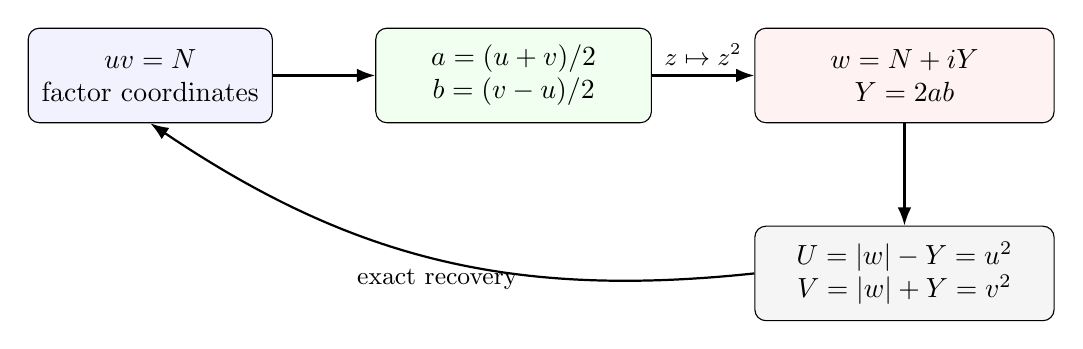
\begin{tikzpicture}[>=Latex,node distance=13mm]
  \node[draw,rounded corners,fill=blue!5,align=center,minimum width=31mm,minimum height=12mm] (factor) {$uv=N$\\factor coordinates};
  \node[draw,rounded corners,fill=green!6,align=center,minimum width=35mm,minimum height=12mm,right=of factor] (fermat) {$a=(u+v)/2$\\$b=(v-u)/2$};
  \node[draw,rounded corners,fill=red!5,align=center,minimum width=38mm,minimum height=12mm,right=of fermat] (square) {$w=N+iY$\\$Y=2ab$};
  \node[draw,rounded corners,fill=gray!8,align=center,minimum width=38mm,minimum height=12mm,below=of square] (null) {$U=|w|-Y=u^2$\\$V=|w|+Y=v^2$};
  \draw[->,thick] (factor) -- (fermat);
  \draw[->,thick] (fermat) -- node[above,font=\small] {$z\mapsto z^2$} (square);
  \draw[->,thick] (square) -- (null);
  \draw[->,thick,bend left=20] (null.west) to node[below,font=\small] {exact recovery} (factor.south);
\end{tikzpicture}
\caption{Equivalent coordinate systems on a complete factor fibre.  The squared coordinates retain the factor pair exactly.}
\label{fig:coordinate-map}
\end{figure}

%======================================================================
\section{The canonical M\"obius point cloud}
\label{sec:canonical-cloud}
%======================================================================

The smooth--transport decomposition does not use every point on each factor fibre.  It selects one canonical point per squarefree source.

For squarefree $m>1$, define
\begin{equation}
 q_m:=\Pplus(m),
 \qquad
 c_m:=\frac{m}{q_m}.
 \label{eq:canonical-cq}
\end{equation}
Unlike the ordered factor pair in \cref{sec:full-fibre}, the canonical pair is not reordered.  The cofactor $c_m$ may exceed $q_m$.  For example,
\[
 m=30,
 \qquad
 q_m=5,
 \qquad
 c_m=6.
\]
Therefore define the signed Fermat coordinate
\begin{equation}
 a_m:=\frac{c_m+q_m}{2},
 \qquad
 b_m:=\frac{q_m-c_m}{2}\in\frac12\Z,
 \label{eq:signed-Fermat}
\end{equation}
and the canonical squared point
\begin{equation}
 w_m:=(a_m+ib_m)^2
 =m+iY_m,
 \label{eq:canonical-w}
\end{equation}
where
\begin{equation}
 \boxed{Y_m=2a_mb_m=\frac{q_m^2-c_m^2}{2}.}
 \label{eq:signed-Y}
\end{equation}
The sign of $Y_m$ records the order of the canonical factors:
\begin{equation}
 Y_m>0\iff c_m<q_m,
 \qquad
 Y_m<0\iff c_m>q_m.
 \label{eq:Y-sign}
\end{equation}

\subsection{Exact parameterization by cofactors and primes}

Every squarefree $m>1$ has a unique representation
\begin{equation}
 m=cq,
 \label{eq:cq-general}
\end{equation}
where
\begin{equation}
 \mu(c)\ne0,
 \qquad
 q\text{ is prime},
 \qquad
 q>\Pplus(c).
 \label{eq:canonical-admissibility}
\end{equation}
Conversely, every pair satisfying \cref{eq:canonical-admissibility} produces a squarefree integer $m=cq$ with largest prime factor $q$.  Moreover,
\begin{equation}
 \mu(cq)=-\mu(c).
 \label{eq:canonical-sign}
\end{equation}

Define the canonical index set
\begin{equation}
 \mathscr C
 :=
 \left\{
 (c,q):
 \mu(c)\ne0,
 \ q\text{ prime},
 \ q>\Pplus(c)
 \right\}.
 \label{eq:canonical-index}
\end{equation}
The squared point cloud is
\begin{equation}
 \mathscr W
 :=
 \left\{
 cq+i\frac{q^2-c^2}{2}:(c,q)\in\mathscr C
 \right\}.
 \label{eq:canonical-cloud}
\end{equation}
The signed point measure is
\begin{equation}
 \nu
 :=
 \delta_1
 -
 \sum_{(c,q)\in\mathscr C}
 \mu(c)\,
 \delta_{\,cq+i(q^2-c^2)/2}.
 \label{eq:signed-measure}
\end{equation}
The atom at $1$ records $\mu(1)=1$.

\begin{example}[A point below the real axis]
For $m=30$, the canonical pair is $(c,q)=(6,5)$, so
\[
 a=\frac{11}{2},
 \qquad
 b=-\frac12,
 \qquad
 w_{30}=30-\frac{11}{2}i.
\]
This point enters a square prefix only after the cutoff already exceeds $q=5$, so it is smooth immediately and never occupies the transport channel.
\end{example}

%======================================================================
\section{Four exact coordinate systems}
\label{sec:coordinates}
%======================================================================

Let
\begin{equation}
 w=x+iy
 =cq+i\frac{q^2-c^2}{2},
 \qquad
 \rho:=|w|=\sqrt{x^2+y^2}.
 \label{eq:w-rho}
\end{equation}
Then
\begin{equation}
 \rho=\frac{c^2+q^2}{2}.
 \label{eq:rho-cq}
\end{equation}
The most useful coordinate charts are collected in \cref{tab:coordinates}.

\begin{table}[htbp]
\centering
\caption{Equivalent coordinates for a canonical squared factor point.}
\label{tab:coordinates}
\renewcommand{\arraystretch}{1.35}
\begin{tabular}{>{\raggedright\arraybackslash}p{0.21\textwidth} >{\raggedright\arraybackslash}p{0.31\textwidth} >{\raggedright\arraybackslash}p{0.34\textwidth}}
\toprule
Coordinate system & Definition & Exact inverse information\\
\midrule
Factor coordinates & $(c,q)$ & $m=cq$, $q=\Pplus(m)$\\
Fermat coordinates & $a=(c+q)/2$, $b=(q-c)/2$ & $c=a-b$, $q=a+b$\\
Squared Cartesian & $x=cq$, $y=(q^2-c^2)/2$ & $w=x+iy=(a+ib)^2$\\
Radial-null & $U=\rho-y$, $V=\rho+y$ & $U=c^2$, $V=q^2$, $x^2=UV$\\
Square-root & $a^2=(\rho+x)/2$, $b^2=(\rho-x)/2$ & sign of $b$ is sign of $y$\\
\bottomrule
\end{tabular}
\end{table}

The central identities are
\begin{equation}
 \boxed{
 U:=\rho-y=c^2,
 \qquad
 V:=\rho+y=q^2.
 }
 \label{eq:UV}
\end{equation}
Consequently,
\begin{equation}
 x=\sqrt{UV}=cq,
 \qquad
 y=\frac{V-U}{2}.
 \label{eq:xy-UV}
\end{equation}

These null coordinates linearize the arithmetic cutoffs.  They also make the meaning of $2ab$ exact:
\begin{equation}
 \boxed{Y=2ab=\frac{V-U}{2},}
 \label{eq:Y-null}
\end{equation}
so the imaginary coordinate is half the separation between the squared canonical factors.

%======================================================================
\section{Cofactor parabolas}
\label{sec:cofactor-curves}
%======================================================================

Fix a positive cofactor $c$ and let $q$ vary.  In squared Cartesian coordinates,
\begin{equation}
 x=cq,
 \qquad
 y=\frac{q^2-c^2}{2}.
 \label{eq:curve-param}
\end{equation}
Eliminating $q=x/c$ gives the cofactor parabola
\begin{equation}
 \boxed{
 \gamma_c(x)
 =\frac{x^2-c^4}{2c^2}.
 }
 \label{eq:gamma-c}
\end{equation}
The canonical point cloud is not the filled region between envelopes.  It is the arithmetic sampling
\begin{equation}
 x=cq,
 \qquad
 q\text{ prime},
 \qquad
 q>\Pplus(c),
 \label{eq:curve-sampling}
\end{equation}
on the family \cref{eq:gamma-c}.

The curve crosses the real axis at
\begin{equation}
 x=c^2.
 \label{eq:curve-axis-cross}
\end{equation}
Points to the right have $q>c$ and positive ordinate; points to the left have $q<c$ and negative ordinate.

The $c=1$ curve is
\begin{equation}
 \gamma_1(x)=\frac{x^2-1}{2}.
 \label{eq:prime-curve}
\end{equation}
Its arithmetic samples are exactly the prime points, since $m=1\cdot q=q$.  It is the outer positive envelope of the complete canonical cloud.  The curve
\begin{equation}
 \gamma_3(x)=\frac{x^2-81}{18}
 \label{eq:three-curve}
\end{equation}
is the first nontrivial odd-cofactor envelope used in semiprime search.

\begin{figure}[htbp]
\centering
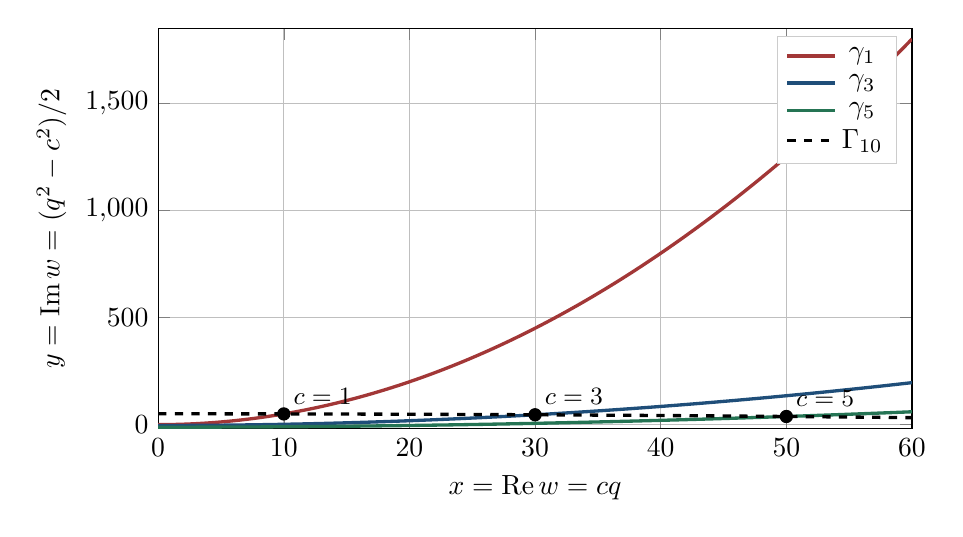
\begin{tikzpicture}
\begin{axis}[
  width=0.92\textwidth,
  height=0.55\textwidth,
  xmin=0,xmax=60,
  ymin=-20,ymax=1850,
  xlabel={$x=\Repart w=cq$},
  ylabel={$y=\Impart w=(q^2-c^2)/2$},
  grid=major,
  legend style={at={(0.98,0.98)},anchor=north east,fill=white,draw=gray!40},
  samples=240,
  domain=0:60,
  clip=true
]
  \addplot[very thick,ovvored] {(x^2-1)/2};
  \addlegendentry{$\gamma_1$}
  \addplot[very thick,ovvoblue] {(x^2-81)/18};
  \addlegendentry{$\gamma_3$}
  \addplot[very thick,ovvogreen] {(x^2-625)/50};
  \addlegendentry{$\gamma_5$}
  \addplot[very thick,black,dashed] {(10000-x^2)/200};
  \addlegendentry{$\Gamma_{10}$}
  \addplot[only marks,mark=*,mark size=2.2pt,black] coordinates {(10,49.5) (30,45.5) (50,37.5)};
  \node[anchor=south west,font=\small] at (axis cs:10,49.5) {$c=1$};
  \node[anchor=south west,font=\small] at (axis cs:30,45.5) {$c=3$};
  \node[anchor=south west,font=\small] at (axis cs:50,37.5) {$c=5$};
\end{axis}
\end{tikzpicture}
\caption{Cofactor parabolas $\gamma_c$ and the moving cutoff parabola $\Gamma_R$ for $R=10$.  Each $\gamma_c$ meets $\Gamma_R$ at $x=cR$.  Actual canonical points are discrete prime samples on the curves.}
\label{fig:cofactor-parabolas}
\end{figure}

%======================================================================
\section{The moving prefix and smoothness cutoff}
\label{sec:moving-cutoff}
%======================================================================

Fix $R>0$.  The complete arithmetic prefix is
\begin{equation}
 \mathscr P_R
 :=\{w=x+iy\in\mathscr W:x<R^2\}.
 \label{eq:prefix-region}
\end{equation}
Since $V=q^2=|w|+y$, the smooth condition $q\le R$ is
\begin{equation}
 |w|+y\le R^2.
 \label{eq:smooth-radial}
\end{equation}
Define
\begin{align}
 \mathscr A_R
 &:={\{w\in\mathscr P_R:|w|+\Impart w\le R^2\}},
 \label{eq:A-region}\\
 \mathscr U_R
 &:={\{w\in\mathscr P_R:|w|+\Impart w>R^2\}}.
 \label{eq:U-region}
\end{align}
The prefix is the disjoint union
\begin{equation}
 \mathscr P_R=\mathscr A_R\,\dot\cup\,\mathscr U_R.
 \label{eq:region-partition}
\end{equation}

Solving \cref{eq:smooth-radial} on the boundary gives
\begin{equation}
 \boxed{
 \Gamma_R(x)=\frac{R^4-x^2}{2R^2}.
 }
 \label{eq:Gamma-R}
\end{equation}
Inside the prefix strip $x<R^2$, the smooth region lies below the graph and the transport region lies above it.

In null coordinates, the same regions are even simpler:
\begin{align}
 \mathscr P_R&:\quad UV<R^4,
 \label{eq:prefix-UV}\\
 \mathscr A_R&:\quad UV<R^4,\quad V\le R^2,
 \label{eq:smooth-UV}\\
 \mathscr U_R&:\quad UV<R^4,\quad V>R^2.
 \label{eq:transport-UV}
\end{align}
For a transport point, $UV<R^4<V^2$, so automatically $U<R^2$.  Thus
\begin{equation}
 \mathscr U_R:\quad U<R^2<V,
 \qquad
 UV<R^4.
 \label{eq:transport-null-clean}
\end{equation}
This is exactly $c<R<q$.

\subsection{Exact intersection with every cofactor curve}

\begin{proposition}[Intersection factorization]
\label{prop:intersection-factorization}
For $c,R>0$,
\begin{equation}
 \gamma_c(x)-\Gamma_R(x)
 =
 \frac{(R^2+c^2)(x^2-c^2R^2)}{2c^2R^2}.
 \label{eq:curve-gap}
\end{equation}
Consequently,
\begin{equation}
 \gamma_c(x)=\Gamma_R(x)
 \iff x=cR.
 \label{eq:curve-intersection}
\end{equation}
At the arithmetic point $x=cq$,
\begin{equation}
 \gamma_c(cq)-\Gamma_R(cq)
 =
 \frac{(R^2+c^2)(q^2-R^2)}{2R^2}.
 \label{eq:point-gap}
\end{equation}
\end{proposition}

The sign is therefore exact:
\begin{align}
 q<R&\iff w_{c,q}\text{ lies below }\Gamma_R,
 \label{eq:below}\\
 q>R&\iff w_{c,q}\text{ lies above }\Gamma_R.
 \label{eq:above}
\end{align}

\begin{proposition}[Orthogonal crossing]
\label{prop:orthogonal-crossing}
At the intersection $x=cR$,
\begin{equation}
 \gamma_c'(cR)=\frac{R}{c},
 \qquad
 \Gamma_R'(cR)=-\frac{c}{R},
 \label{eq:orthogonal-slopes}
\end{equation}
so
\begin{equation}
 \gamma_c'(cR)\Gamma_R'(cR)=-1.
 \label{eq:orthogonal-product}
\end{equation}
Hence each cofactor curve meets the moving cutoff orthogonally.
\end{proposition}

The transition is therefore transverse, never tangent.  A canonical point cannot remain trapped in a thin boundary layer as the cutoff passes its largest prime.

%======================================================================
\section{The exact moving-region form of $A-T$}
\label{sec:moving-region-AT}
%======================================================================

Using the signed measure \cref{eq:signed-measure}, define
\begin{equation}
 \mathcal A(R):=\nu(\mathscr A_R),
 \qquad
 \mathcal U(R):=\nu(\mathscr U_R).
 \label{eq:AU-measures}
\end{equation}
At $R=R_n$,
\begin{equation}
 \mathcal A(R_n)=A_n,
 \qquad
 \mathcal U(R_n)=-T_n.
 \label{eq:AU-AT}
\end{equation}
Indeed, the transport points satisfy $c<R_n<q$ and carry signed point mass
\[
 \mu(cq)=-\mu(c).
\]
Therefore
\begin{equation}
 \boxed{
 S_n
 =\nu(\mathscr P_{R_n})
 =\mathcal A(R_n)+\mathcal U(R_n)
 =A_n-T_n.
 }
 \label{eq:geometric-AT}
\end{equation}

Equivalently, define projectors
\begin{align}
 P_R(w)&:=\1_{\{\Repart w<R^2\}},
 \label{eq:P-projector}\\
 Q_R(w)&:=\1_{\{|w|+\Impart w\le R^2\}}.
 \label{eq:Q-projector}
\end{align}
Then
\begin{align}
 \mathcal A(R)&=\int P_RQ_R\,d\nu,
 \label{eq:A-projector}\\
 \mathcal U(R)&=\int P_R(1-Q_R)\,d\nu,
 \label{eq:U-projector}\\
 S(R)&=\int P_R\,d\nu.
 \label{eq:S-projector}
\end{align}
The identity is the pointwise partition
\begin{equation}
 P_R=P_RQ_R+P_R(1-Q_R).
 \label{eq:projector-partition}
\end{equation}

%======================================================================
\section{Entry time, transition time, and exact telescoping}
\label{sec:telescoping}
%======================================================================

For a canonical source $m=cq$, define its first square-prefix index
\begin{equation}
 e(m):=\lfloor\sqrt m\rfloor.
 \label{eq:entry-index}
\end{equation}
This is the least $n$ such that $m<R_n^2$.  Define the smoothness-transition index
\begin{equation}
 h(m):=q-1.
 \label{eq:transition-index}
\end{equation}
This is the least $n$ such that $q\le R_n$.

The transport lifetime is
\begin{equation}
 L(m):=(h(m)-e(m))_+.
 \label{eq:lifetime}
\end{equation}
There are two cases:

\begin{enumerate}[leftmargin=1.7em,itemsep=0.3em]
\item If $q>\sqrt m$, equivalently $q>c$ and $Y>0$, then the point enters above the moving parabola and occupies transport for the discrete interval
\[
 e(m)\le n<h(m).
\]
\item If $q\le\sqrt m$, equivalently $q\le c$ and $Y\le0$, then $h(m)\le e(m)$ and the point enters already smooth.  Its transport interval is empty.
\end{enumerate}

Define the pointwise indicators
\begin{align}
 p_n(m)&:=\1_{\{e(m)\le n\}},
 \label{eq:p-indicator}\\
 u_n(m)&:=\1_{\{e(m)\le n<h(m)\}},
 \label{eq:u-indicator}\\
 a_n(m)&:=\1_{\{e(m)\le n,\ h(m)\le n\}}.
 \label{eq:a-indicator}
\end{align}
Then
\begin{equation}
 \boxed{p_n(m)=u_n(m)+a_n(m).}
 \label{eq:temporal-partition}
\end{equation}

\subsection{Crossing cancellation}

Let $E_n^A$ be the signed mass entering the new vertical strip already below the moving parabola, let $E_n^U$ be the signed mass entering above it, and let $C_n$ be the signed mass crossed by the moving parabola between $R_{n-1}$ and $R_n$.  Then
\begin{align}
 \mathcal A(R_n)-\mathcal A(R_{n-1})
 &=E_n^A+C_n,
 \label{eq:Delta-A}\\
 \mathcal U(R_n)-\mathcal U(R_{n-1})
 &=E_n^U-C_n.
 \label{eq:Delta-U}
\end{align}
Therefore
\begin{equation}
 \boxed{
 S_n-S_{n-1}
 =E_n^A+E_n^U
 =\sum_{m\in B_n}\mu(m).
 }
 \label{eq:Delta-S}
\end{equation}
The entire crossing mass cancels.

\begin{figure}[htbp]
\centering
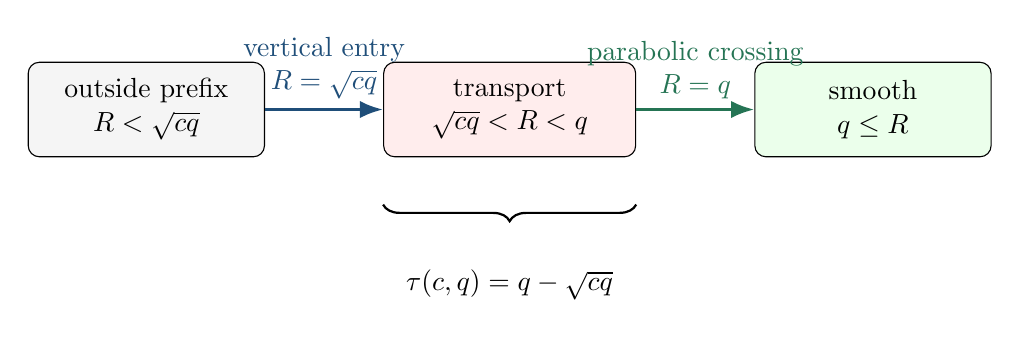
\begin{tikzpicture}[>=Latex,node distance=15mm]
  \node[draw,rounded corners,fill=gray!8,minimum width=30mm,minimum height=12mm,align=center] (out) {outside prefix\\$R<\sqrt{cq}$};
  \node[draw,rounded corners,fill=red!7,minimum width=32mm,minimum height=12mm,align=center,right=of out] (trans) {transport\\$\sqrt{cq}<R<q$};
  \node[draw,rounded corners,fill=green!8,minimum width=30mm,minimum height=12mm,align=center,right=of trans] (smooth) {smooth\\$q\le R$};
  \draw[->,very thick,ovvoblue] (out) -- node[above,align=center] {vertical entry\\$R=\sqrt{cq}$} (trans);
  \draw[->,very thick,ovvogreen] (trans) -- node[above,align=center] {parabolic crossing\\$R=q$} (smooth);
  \draw[decorate,decoration={brace,amplitude=6pt,mirror},thick] ($(trans.south west)+(0,-6mm)$) -- ($(trans.south east)+(0,-6mm)$) node[midway,below=7mm] {$\tau(c,q)=q-\sqrt{cq}$};
\end{tikzpicture}
\caption{The exact state path of a positive-height canonical point.  The second transition only reallocates signed mass between $-T$ and $A$, so it cancels from the residual increment.}
\label{fig:state-path}
\end{figure}

This is the telescopic nature of the squared coordinate: the point's imaginary height determines when the moving parabola reaches it, while the crossing itself contributes zero to the increment of the total prefix mass.

%======================================================================
\section{The exact $2ab$ lifetime law}
\label{sec:lifetime-law}
%======================================================================

Define the signed continuous delay
\begin{equation}
 \tau(c,q):=q-\sqrt{cq}.
 \label{eq:tau}
\end{equation}
It is positive exactly for transport-capable points, zero at $c=q$, and negative for points that enter already smooth.

Put
\begin{equation}
 r:=\frac cq.
 \label{eq:r-ratio}
\end{equation}
Then
\begin{equation}
 Y=\frac{q^2}{2}(1-r^2)
 \label{eq:Y-r}
\end{equation}
and
\begin{equation}
 \tau=q(1-\sqrt r).
 \label{eq:tau-r}
\end{equation}
Since
\begin{equation}
 1-r^2=(1-\sqrt r)(1+\sqrt r)(1+r),
 \label{eq:factor-r}
\end{equation}
we obtain an exact identity.

\begin{theorem}[Exact height--lifetime identity]
\label{thm:exact-height-lifetime}
For every positive pair $(c,q)$,
\begin{equation}
 \boxed{
 Y
 =
 \frac{q\tau}{2}
 \left(1+\sqrt{\frac cq}\right)
 \left(1+\frac cq\right).
 }
 \label{eq:Y-tau-exact}
\end{equation}
Equivalently,
\begin{equation}
 \boxed{
 \tau
 =
 \frac{2Y}
 {q\left(1+\sqrt{c/q}\right)\left(1+c/q\right)}.
 }
 \label{eq:tau-Y-exact}
\end{equation}
\end{theorem}

The sign of $Y$ is therefore exactly the sign of the continuous delay.  On the transport side $0<c/q<1$, the denominator in \cref{eq:tau-Y-exact} lies between $q$ and $4q$, giving
\begin{equation}
 \frac{Y}{2q}
 \le\tau
 \le\frac{2Y}{q}.
 \label{eq:tau-bounds}
\end{equation}
Since
\begin{equation}
 L(m)=q-1-\lfloor\sqrt m\rfloor
 \le q-\sqrt m=\tau(c,q)
 \label{eq:L-tau}
\end{equation}
for transport points,
\begin{equation}
 \boxed{L(m)\le\frac{2Y_m}{q_m}.}
 \label{eq:L-Y}
\end{equation}

In squared-space coordinates, $q=\sqrt{|w|+\Impart w}$, so
\begin{equation}
 L(w)
 \le
 \frac{2(\Impart w)_+}
 {\sqrt{|w|+\Impart w}}.
 \label{eq:L-w}
\end{equation}
A point close to the real axis cannot remain in transport for many prefix steps.

%======================================================================
\section{Low-height clustering in real square strips}
\label{sec:clustering}
%======================================================================

The $n$th square block becomes the vertical strip
\begin{equation}
 \mathscr B_n
 :=\{w_m:n^2\le\Repart w_m<(n+1)^2\}.
 \label{eq:complex-block}
\end{equation}
For a canonical pair $(c,q)$, define the absolute factor gap
\begin{equation}
 d:=|q-c|.
 \label{eq:absolute-gap}
\end{equation}
Then
\begin{equation}
 |Y|
 =\frac{|q^2-c^2|}{2}
 =\frac{d(q+c)}{2}.
 \label{eq:Y-absolute-gap}
\end{equation}
For a squarefree source $m>1$, one has $d\ge1$: equality $d=0$ would
force $m=c^2$.

\begin{lemma}[At most one product per positive absolute gap]
\label{lem:one-product-gap}
Fix $n\ge1$ and an integer $d\ge1$.  There is at most one unordered
positive factor pair $\{c,q\}$ with $|q-c|=d$ and
\begin{equation}
 n^2\le cq<(n+1)^2.
 \label{eq:gap-block-condition}
\end{equation}
\end{lemma}

\begin{proof}
Write the smaller factor as $r$ and the larger as $r+d$.  The product is
$f_d(r)=r(r+d)$.  If $f_d(r)\in B_n$, then
\[
 2r+d\ge2\sqrt{r(r+d)}\ge2n.
\]
Hence
\[
 f_d(r+1)-f_d(r)=2r+d+1\ge2n+1,
\]
which exceeds the integer diameter $2n$ of the block.  Thus two
distinct values of $r$ cannot both occur.
\end{proof}

\begin{theorem}[Sharpened absolute low-height clustering]
\label{thm:absolute-clustering}
For every $H\ge0$,
\begin{equation}
 \boxed{
 \#\{w_m\in\mathscr B_n:|Y_m|\le H\}
 \le
 \left\lfloor\frac{H}{n}\right\rfloor.
 }
 \label{eq:absolute-clustering}
\end{equation}
Moreover,
\begin{equation}
 \boxed{
 \#\{w_m\in\mathscr B_n:|Y_m|\le n\}=0.
 }
 \label{eq:no-height-n-points}
\end{equation}
\end{theorem}

\begin{proof}
If $cq\in B_n$, then
\[
 c+q\ge2\sqrt{cq}\ge2n.
\]
Therefore
\[
 |Y|=\frac{d(c+q)}2\ge dn.
\]
The condition $|Y|\le H$ implies
$d\le\lfloor H/n\rfloor$.  Since $d\ge1$, there are at most
$\lfloor H/n\rfloor$ possible gaps, and
\cref{lem:one-product-gap} gives at most one point for each gap.

If $|Y|\le n$, the inequalities force $d=1$ and $c+q=2n$.
But $|q-c|=1$ makes $c+q$ odd, whereas $2n$ is even.  Hence equality is
impossible and the set is empty.
\end{proof}

\subsection{Parity-refined bounds}

The factor gap has a prescribed parity:
\begin{itemize}[leftmargin=1.7em]
\item if $m$ is odd, then $c$ and $q$ are odd, so $d$ is even;
\item if $m$ is even and squarefree, then the canonical factors have
      opposite parity, so $d$ is odd.
\end{itemize}
Let
\begin{equation}
 D:=\left\lfloor\frac{H}{n}\right\rfloor.
 \label{eq:D-height}
\end{equation}
The permitted positive gaps are therefore
\[
 2,4,\ldots,2\left\lfloor\frac D2\right\rfloor
\]
for odd sources and
\[
 1,3,\ldots,2\left\lceil\frac D2\right\rceil-1
\]
for even sources.  Consequently,
\begin{align}
 \#\{w_m\in\mathscr B_n:m\text{ odd},\ |Y_m|\le H\}
 &\le
 \left\lfloor\frac{H}{2n}\right\rfloor,
 \label{eq:odd-parity-clustering}\\
 \#\{w_m\in\mathscr B_n:m\text{ even},\ |Y_m|\le H\}
 &\le
 \left\lceil\frac{1}{2}
 \left\lfloor\frac{H}{n}\right\rfloor\right\rceil.
 \label{eq:even-parity-clustering}
\end{align}
At the endpoint $H=n$, both populations are empty by
\cref{eq:no-height-n-points}.

At height $H=\Lambda n$, the scale-free bounds become
\begin{align}
 \#\{w_m\in\mathscr B_n:|Y_m|\le\Lambda n\}
 &\le\lfloor\Lambda\rfloor,
 \label{eq:constant-occupancy}\\
 \#\{m\text{ odd}:|Y_m|\le\Lambda n\}
 &\le\left\lfloor\frac{\Lambda}{2}\right\rfloor.
 \label{eq:constant-odd-occupancy}
\end{align}

\subsection{Sharpened low-height space--time budget}

For negative-height points, the transport lifetime is zero.  For
positive-height points in $\mathscr B_n$, one has
$q\ge\sqrt m\ge n$, so \cref{eq:L-Y} gives
\begin{equation}
 L(m)\le\frac{2H}{n}
 \qquad(0<Y_m\le H).
 \label{eq:L-H-n}
\end{equation}
Therefore
\begin{equation}
 \boxed{
 \sum_{\substack{w_m\in\mathscr B_n\\|Y_m|\le H}}
 (1+L(m))
 \le
 \left\lfloor\frac{H}{n}\right\rfloor
 \left(1+\frac{2H}{n}\right).
 }
 \label{eq:space-time-budget}
\end{equation}
The parity-refined versions are
\begin{align}
 \sum_{\substack{w_m\in\mathscr B_n\\m\text{ odd},\ |Y_m|\le H}}
 (1+L(m))
 &\le
 \left\lfloor\frac{H}{2n}\right\rfloor
 \left(1+\frac{2H}{n}\right),
 \label{eq:odd-space-time-budget}\\
 \sum_{\substack{w_m\in\mathscr B_n\\m\text{ even},\ |Y_m|\le H}}
 (1+L(m))
 &\le
 \left\lceil\frac{1}{2}
 \left\lfloor\frac{H}{n}\right\rfloor\right\rceil
 \left(1+\frac{2H}{n}\right).
 \label{eq:even-space-time-budget}
\end{align}
At $H=\Lambda n$, all three right sides are bounded independently of
$n$.

%======================================================================
\section{The quadratic map is conformal and supplies two powers}
\label{sec:jacobian}
%======================================================================

Consider the continuous map
\begin{equation}
 \Phi(c,q)
 :=
 \left(
 x(c,q),y(c,q)
 \right)
 =
 \left(
 cq,\frac{q^2-c^2}{2}
 \right).
 \label{eq:Phi}
\end{equation}
Its differential is
\begin{equation}
 D\Phi(c,q)
 =
 \begin{pmatrix}
 q & c\\
 -c & q
 \end{pmatrix}.
 \label{eq:D-Phi}
\end{equation}
The two columns are orthogonal and have equal length $\sqrt{c^2+q^2}$.  Consequently,
\begin{equation}
 D\Phi(c,q)^{\mathsf T}D\Phi(c,q)
 =(c^2+q^2)I.
 \label{eq:conformal-metric}
\end{equation}
Thus $\Phi$ is conformal: locally it rotates and expands every direction by the same factor
\begin{equation}
 \lambda(c,q)=\sqrt{c^2+q^2}.
 \label{eq:length-scale}
\end{equation}
The area Jacobian is
\begin{equation}
 \boxed{
 J(c,q)=\det D\Phi(c,q)=c^2+q^2=2|w|.
 }
 \label{eq:Jacobian}
\end{equation}
By AM--GM,
\begin{equation}
 c^2+q^2\ge2cq=2x.
 \label{eq:Jacobian-lower}
\end{equation}
Therefore, in the square strip $x\asymp n^2$,
\begin{equation}
 \lambda(c,q)\gtrsim n,
 \qquad
 J(c,q)\gtrsim n^2.
 \label{eq:square-scale-expansion}
\end{equation}

This is the two-dimensional version of the vertical spacing estimate.  Unit-scale separation in the factor plane becomes scale-$n$ separation in the squared plane, while unit factor-lattice area becomes scale-$n^2$ area.  The coherent square-prefix ceiling loses exactly two powers if the relevant kernel neighborhoods have bounded squared-space area after localization.

\begin{caution}[What the Jacobian does not prove]
The M\"obius point cloud is discrete and arithmetically restricted, and the square-prefix kernel is not Euclidean convolution.  The Jacobian therefore does not by itself prove a signed variance estimate.  It proves the exact geometric dilution scale that a valid operator argument must inherit.
\end{caution}


\subsection{Two-dimensional area versus one-dimensional cofactor curves}
\label{subsec:curve-versus-area}

The conformal Jacobian governs two-dimensional regions in the continuous
$(c,q)$ factor plane.  The arithmetic measure is not two-dimensional:
for each fixed cofactor $c$, it is supported on the one-dimensional
prime-sampled curve
\[
 q\longmapsto
 \Phi(c,q)
 =
 \left(cq,\frac{q^2-c^2}{2}\right),
 \qquad
 q\ \text{prime},\quad q>\Pplus(c).
\]
Along that curve,
\begin{equation}
 \left\lVert\frac{\partial\Phi}{\partial q}(c,q)\right\rVert
 =
 \sqrt{c^2+q^2}.
 \label{eq:curve-length-expansion}
\end{equation}
Thus one-dimensional arclength is also expanded, but the number and
arithmetic placement of samples are governed by primes rather than by
the area Jacobian.  A two-dimensional density estimate cannot be
applied directly to a single cofactor curve.

The outer curve $c=1$ makes this obstruction explicit.  Its contribution
to the $n$th complete prefix is
\begin{equation}
 S_n^{(1)}
 =
 -\pi(X_n),
 \label{eq:prime-curve-prefix}
\end{equation}
because every prime $q\le X_n$ has canonical pair $(1,q)$ and M\"obius
weight $-1$.  The prime number theorem therefore predicts
\begin{equation}
 \sum_{n\le N}|S_n^{(1)}|^2
 \sim
 \frac{N^5}{20\log^2 N},
 \label{eq:prime-curve-asymptotic}
\end{equation}
up to the usual slowly varying correction.  The prime curve by itself
is not on the cubic scale.  Cancellation between $c=1$ and the
aggregate of the curves $c\ge2$ is indispensable.

This also shows why a bound of the form
\[
 \sum_{q\le Q}e\!\left(\alpha\frac{q^2-c^2}{2}\right)
 \ll Q^{1/2+\eps}
\]
cannot hold uniformly in $\alpha$: at $\alpha=0$ the left side is
$\pi(Q)+O(1)$.  The zero and major-arc modes must be cancelled across
cofactor curves by the M\"obius weights $\mu(c)$ and the exact
smooth--transport architecture.  Oscillatory estimates are relevant
only after that coherent component has been isolated.

\begin{definition}[Dyadic squared-cofactor exponential sum]
\label{def:squared-cofactor-sum}
For dyadic $C,Q\ge1$, define
\begin{equation}
 F_{C,Q}(\alpha)
 :=
 \sum_{\substack{C<c\le2C\\\mu(c)\ne0}}
 -\mu(c)e\!\left(-\alpha\frac{c^2}{2}\right)
 \sum_{\substack{Q<q\le2Q\\q\ {\rm prime}\\q>\Pplus(c)}}
 e\!\left(\alpha\frac{q^2}{2}\right).
 \label{eq:F-CQ}
\end{equation}
\end{definition}

A concrete analytic route is a major/minor-arc decomposition for
$F_{C,Q}$, coupled to the Fourier representation of localized
squared-space kernels.  The major arcs must reproduce and cancel the
coherent cofactor-curve main terms, while the minor arcs must satisfy a
large-sieve or mean-square estimate.  This is the analytic content that
the conformal geometry identifies but does not itself prove.

%======================================================================
\section{Vertical spacing on a fixed real fibre}
\label{sec:vertical-spacing}
%======================================================================

Fix $m>0$ and parameterize the full factor hyperbola by signed $b\in\R$:
\begin{equation}
 a=\sqrt{m+b^2},
 \qquad
 Y_m(b)=2b\sqrt{m+b^2}.
 \label{eq:Y-b}
\end{equation}
Then
\begin{equation}
 Y_m'(b)
 =2\frac{m+2b^2}{\sqrt{m+b^2}}
 \ge2\sqrt m.
 \label{eq:Y-derivative}
\end{equation}
The derivative is positive for all signed $b$, so the map is strictly increasing from the lower to the upper half-plane.

If admissible $b$ values differ by at least $h$, then
\begin{equation}
 |\Delta Y|\ge2h\sqrt m.
 \label{eq:Y-spacing}
\end{equation}
At square scale $m\asymp n^2$, vertical spacing is at least order $n$.  This agrees with the conformal scale factor in \cref{eq:square-scale-expansion}.

%======================================================================
\section{The square-prefix variance as a squared-space kernel}
\label{sec:variance-kernel}
%======================================================================

For a canonical point $w_m$, define
\begin{equation}
 p_n(w_m):=\1_{\{e(m)\le n\}}.
 \label{eq:prefix-indicator}
\end{equation}
Then
\begin{equation}
 S_n=\int p_n(w)\,d\nu(w).
 \label{eq:S-integral}
\end{equation}
For a terminal index $N$, define
\begin{equation}
 K_N(w,w')
 :=\sum_{n=1}^{N}p_n(w)p_n(w').
 \label{eq:prefix-kernel}
\end{equation}
Since each $p_n$ is a tail indicator,
\begin{equation}
 K_N(w,w')
 =
 \bigl(N-\max\{e(w),e(w')\}+1\bigr)_+.
 \label{eq:prefix-kernel-explicit}
\end{equation}
Therefore
\begin{equation}
 \boxed{
 \sum_{n=1}^{N}|S_n|^2
 =
 \iint_{\mathscr W\times\mathscr W}
 K_N(w,w')\,d\nu(w)d\nu(w').
 }
 \label{eq:variance-kernel}
\end{equation}

The channel indicators satisfy
\begin{equation}
 p_n=a_n+u_n,
 \label{eq:channel-indicator-sum}
\end{equation}
so the kernel splits exactly into smooth--smooth, transport--transport, and two cross terms.

For transport, the overlap kernel has the interval form
\begin{equation}
 K_N^{UU}(w,w')
 =
 \#\left(
 [e(w),h(w))
 \cap
 [e(w'),h(w'))
 \cap
 [1,N]
 \right).
 \label{eq:transport-overlap}
\end{equation}
Consequently,
\begin{equation}
 K_N^{UU}(w,w')
 \le\min\{L(w),L(w')\}.
 \label{eq:transport-overlap-bound}
\end{equation}
The imaginary coordinate therefore controls temporal support through \cref{eq:L-w}.

%======================================================================
\section{A rigorous cubic bound for the low-height sector}
\label{sec:low-cubic}
%======================================================================

Fix $\Lambda>0$.  Assign each source $m$ to its entry block
\begin{equation}
 j=e(m)=\lfloor\sqrt m\rfloor
 \label{eq:entry-block}
\end{equation}
and define the low-height block increment
\begin{equation}
 d_j^{\mathrm{low}}
 :=
 \sum_{\substack{m\in B_j\\|Y_m|\le\Lambda j}}
 \mu(m).
 \label{eq:low-block-increment}
\end{equation}
By \cref{eq:constant-occupancy},
\begin{equation}
 |d_j^{\mathrm{low}}|
 \le\lfloor\Lambda\rfloor.
 \label{eq:low-block-bound}
\end{equation}
Define
\begin{equation}
 S_n^{\mathrm{low}}
 :=\sum_{j\le n}d_j^{\mathrm{low}}.
 \label{eq:low-prefix}
\end{equation}
Even under complete sign coherence,
\begin{equation}
 |S_n^{\mathrm{low}}|
 \le\lfloor\Lambda\rfloor n.
 \label{eq:low-prefix-bound}
\end{equation}
Hence
\begin{equation}
 \boxed{
 \sum_{n\le N}|S_n^{\mathrm{low}}|^2
 \ll_{\Lambda}N^3.
 }
 \label{eq:low-cubic}
\end{equation}
No M\"obius cancellation is used.

Let
\begin{equation}
 S_n=S_n^{\mathrm{low}}+S_n^{\mathrm{high}}.
 \label{eq:low-high-split}
\end{equation}
Then
\begin{equation}
 \sum_{n\le N}|S_n|^2
 \le
 2\sum_{n\le N}|S_n^{\mathrm{low}}|^2
 +
 2\sum_{n\le N}|S_n^{\mathrm{high}}|^2.
 \label{eq:energy-low-high}
\end{equation}
Thus the low-height sector is already on the cubic scale.  The entire unresolved variance problem may be localized to the high-height point cloud.

%======================================================================
\section{The high-height cofactor-curve problem}
\label{sec:high-sector}
%======================================================================

The high sector consists of canonical points satisfying
\begin{equation}
 |Y_m|>\Lambda e(m).
 \label{eq:high-sector}
\end{equation}
These points lie far from the real axis relative to their square scale,
but they remain highly structured:

\begin{enumerate}[leftmargin=1.7em,itemsep=0.3em]
\item they lie on the explicit curves $\gamma_c$;
\item their horizontal coordinates are prime samples $x=cq$ with
      $q>\Pplus(c)$;
\item their one-dimensional curve spacing is expanded by
      $\sqrt{c^2+q^2}$;
\item two-dimensional factor regions are expanded by
      $c^2+q^2$;
\item positive-height points have exact transport intervals
      $[e(m),h(m))$;
\item each curve crosses every moving cutoff exactly once and
      orthogonally.
\end{enumerate}

For each squarefree cofactor $c$, define the signed curve measure
\begin{equation}
 \nu_c
 :=
 -\mu(c)
 \sum_{\substack{q\text{ prime}\\q>\Pplus(c)}}
 \delta_{\,cq+i(q^2-c^2)/2}.
 \label{eq:nu-c}
\end{equation}
Then
\begin{equation}
 \nu=\delta_1+\sum_{c\ge1}\nu_c,
 \label{eq:nu-curve-sum}
\end{equation}
and the variance decomposes as
\begin{equation}
 \sum_{c,c'}
 \iint K_N(w,w')\,d\nu_c(w)d\nu_{c'}(w').
 \label{eq:curve-interactions}
\end{equation}

The curve $c=1$ is not a negligible boundary case.  By
\cref{eq:prime-curve-prefix,eq:prime-curve-asymptotic}, its unsigned
energy is of order $N^5/\log^2N$.  The cubic residual therefore requires
near-complete cancellation between this prime curve and the remaining
cofactor curves.  The numerical results in \cref{sec:numerics} measure
that cancellation directly.

\subsection{A precise kernel-weighted large-sieve target}

Fix a local prefix interval
\begin{equation}
 I=[N,N+H),
 \qquad 1\le H\le N,
 \label{eq:local-prefix-I}
\end{equation}
and dyadic ranges $C<c\le2C$, $Q<q\le2Q$.  Let
$\omega_{I,\ell}(c,q)$ be a smooth localization to the prefix interval,
the transport interval, and a high vertical shell $\ell$.  Define
\begin{equation}
 F_{C,Q,\ell}^{I}(\alpha)
 :=
 \sum_{\substack{C<c\le2C\\\mu(c)\ne0}}
 -\mu(c)e\!\left(-\alpha\frac{c^2}{2}\right)
 \sum_{\substack{Q<q\le2Q\\q\text{ prime}\\q>\Pplus(c)}}
 \omega_{I,\ell}(c,q)
 e\!\left(\alpha\frac{q^2}{2}\right).
 \label{eq:F-CQ-local}
\end{equation}
Let $\widehat K_{I,\ell}(\alpha)\ge0$ be the Fourier multiplier of the
corresponding localized positive semidefinite prefix/transport-overlap
kernel.

For parameters $R_0,\Delta\ge1$, define the major arcs
\begin{equation}
 \mathfrak M(R_0,\Delta)
 :=
 \bigcup_{1\le r\le R_0}
 \bigcup_{\substack{0\le a<r\\(a,r)=1}}
 \left\{
 \alpha\in\mathbb R/\mathbb Z:
 \left|\alpha-\frac ar\right|
 \le\frac{\Delta}{rN^2}
 \right\}.
 \label{eq:major-arcs}
\end{equation}
For $\alpha=a/r+\beta$ on such an arc, define the explicit
Hardy--Littlewood model by replacing the prime indicator in
\cref{eq:F-CQ-local} with its reduced-residue main term:
\begin{align}
 \mathcal M_{C,Q,\ell}^{I}(\alpha)
 &:={}
 \sum_{\substack{C<c\le2C\\\mu(c)\ne0}}
 -\mu(c)e\!\left(-\alpha\frac{c^2}{2}\right)
 \frac{G_r(a)}{\varphi(r)}
 \int_Q^{2Q}
 \omega_{I,\ell}(c,t)
 e\!\left(\beta\frac{t^2}{2}\right)
 \frac{dt}{\log t},
 \label{eq:major-arc-model}\\
 G_r(a)
 &:={}
 \sum_{\substack{u\bmod r\\(u,r)=1}}
 e\!\left(\frac{au^2}{2r}\right).
 \label{eq:quadratic-Gauss-prime}
\end{align}
Outside $\mathfrak M(R_0,\Delta)$, put
$\mathcal M_{C,Q,\ell}^{I}=0$.

\begin{conjecture}[Kernel-weighted Squared-Cofactor Large Sieve]
\label{conj:squared-cofactor-large-sieve}
For every $\eps>0$, there are choices
$R_0=N^{o(1)}$ and $\Delta=N^{o(1)}$ such that, uniformly for
$1\le H\le N$,
\begin{align}
 &\sum_{C,Q,\ell}
 \int_{\mathbb R/\mathbb Z}
 \left|
 F_{C,Q,\ell}^{I}(\alpha)
 -\mathcal M_{C,Q,\ell}^{I}(\alpha)
 \right|^2
 \widehat K_{I,\ell}(\alpha)\,d\alpha
 \ll_\eps HN^{2+\eps},
 \label{eq:cofactor-large-sieve-remainder}\\
 &\int_{\mathbb R/\mathbb Z}
 \left|
 \sum_{C,Q,\ell}
 \mathcal M_{C,Q,\ell}^{I}(\alpha)
 \right|^2
 \widehat K_I(\alpha)\,d\alpha
 \ll_\eps HN^{2+\eps}.
 \label{eq:cofactor-large-sieve-major}
\end{align}
The dyadic sums range only over cells meeting the high sector and the
prefix interval, and the localized multipliers satisfy
$\sum_\ell\widehat K_{I,\ell}\ll\widehat K_I$.
\end{conjecture}

The first estimate is the kernel-weighted minor-arc and major-arc error
bound.  The second is the required cancellation of the explicit
major-arc models across cofactor scales.  Both clauses are necessary:
at zero frequency the prime curve is of order $\pi(Q)$, so a uniform
pointwise square-root estimate is false.  The conjecture places the
large-sieve assertion exactly in the norm generated by the
square-prefix kernel rather than in an unrelated collision statistic.

\begin{conjecture}[High cofactor-curve kernel estimate]
\label{conj:high-kernel}
After removing the low-height sector controlled by
\cref{eq:low-cubic}, the signed cofactor-curve interactions satisfy,
for every $\eps>0$,
\begin{equation}
 \sum_{n\le N}|S_n^{\mathrm{high}}|^2
 \ll_{\eps,\Lambda}N^{3+\eps}.
 \label{eq:high-kernel-bound}
\end{equation}
The two clauses of Conjecture~\ref{conj:squared-cofactor-large-sieve}
are a sufficient analytic route: the first controls the localized
remainder and the second controls the cofactor-cancelled major-arc
model.
\end{conjecture}

This formulation is stronger than rewriting RH in the coordinate $Y$.
It asks for separate control of cofactor ranges, prime ranges,
squared-space shells, and transport-overlap multipliers.  It also
identifies the precise analytic obstruction: a one-dimensional
prime-sampled large sieve coupled across the M\"obius-weighted family of
cofactor parabolas.

%======================================================================

\section{Exponent accounting in squared complex space}
\label{sec:exponent-accounting}
%======================================================================

The block increment
\begin{equation}
 d_n=S_n-S_{n-1}
 \label{eq:d-n}
\end{equation}
satisfies the trivial bound $|d_n|\le2n+1$.  Expanding the cumulative energy gives
\begin{equation}
 \sum_{n\le N}|S_n|^2
 =
 \sum_{j,k\le N}
 \bigl(N-\max\{j,k\}+1\bigr)d_jd_k.
 \label{eq:triangular-energy}
\end{equation}
The fully coherent ceiling is
\begin{equation}
 N^5
 =
 \underbrace{N}_{\text{prefix multiplicity}}
 \times
 \underbrace{N^2}_{\text{block pairs}}
 \times
 \underbrace{N^2}_{\text{raw pair amplitude}}.
 \label{eq:N5-accounting}
\end{equation}

The squared map provides the exact missing scale:
\begin{equation}
 J(c,q)=c^2+q^2\ge2cq\asymp n^2.
 \label{eq:two-power-J}
\end{equation}
Thus a unit area of factor combinations is diluted by $n^{-2}$ in the squared plane.  Equivalently, each coordinate direction is stretched by order $n$.  If the localized kernel respects this conformal dilution, then the effective pair amplitude becomes order one:
\begin{equation}
 N^3
 =
 \underbrace{N}_{\text{prefix multiplicity}}
 \times
 \underbrace{N^2}_{\text{block pairs}}
 \times
 \underbrace{1}_{\text{squared-space interaction}}.
 \label{eq:N3-accounting}
\end{equation}

The low-height theorem proves this reduction directly in the region $|Y|\lesssim n$.  The high-height conjecture asks for the corresponding operator statement in the remaining region.

%======================================================================
\section{A uniform local criterion for RH}
\label{sec:local-criterion}
%======================================================================

The global cubic energy is the natural benchmark, but a fully pointwise converse is obtained from a uniform local estimate.  Define
\begin{equation}
 V_{\mathrm{loc}}(N,H)
 :=\sum_{n=N}^{N+H-1}|S_n|^2.
 \label{eq:Vloc}
\end{equation}

\begin{theorem}[Uniform local square-prefix criterion]
\label{thm:local-RH}
The Riemann Hypothesis is equivalent to the statement that, for every $\eps>0$,
\begin{equation}
 V_{\mathrm{loc}}(N,H)
 \ll_\eps HN^{2+\eps}
 \qquad(1\le H\le N).
 \label{eq:local-RH}
\end{equation}
\end{theorem}

\begin{proof}
Under RH, the classical Mertens criterion gives
\[
 M(x)\ll_\delta x^{1/2+\delta}
\]
for every $\delta>0$.  Since $X_n\asymp n^2$, one has
\[
 |S_n|^2\ll_\eps n^{2+\eps},
\]
and summing $H$ consecutive terms gives \cref{eq:local-RH}.

Conversely, set $H=1$.  Then
\[
 |S_N|^2\ll_\eps N^{2+\eps},
\]
so $|S_N|\ll_\eta N^{1+\eta}$ for every $\eta>0$.  If
\[
 n^2\le x<(n+1)^2,
\]
then
\[
 |M(x)-M(n^2-1)|\le2n+1
\]
because $|\mu(m)|\le1$.  Therefore
\[
 M(x)\ll_\eta x^{1/2+\eta},
\]
which is equivalent to RH.
\end{proof}

A local version of \cref{conj:high-kernel} would therefore complete the argument without relying on a global-average converse.

%======================================================================
\section{Numerical results and pre-registered diagnostics}
\label{sec:numerics}
%======================================================================

The computations reported here use exact integer arithmetic through
\begin{equation}
 N_{\max}=4096,
 \qquad
 X_{\max}=(4097)^2-1=16{,}785{,}408.
 \label{eq:numerical-range}
\end{equation}
A linear sieve produced
\begin{equation}
 1{,}078{,}362\ \text{primes}
 \qquad\text{and}\qquad
 10{,}204{,}280\ \text{squarefree sources }m\ge2.
 \label{eq:numerical-counts}
\end{equation}

\subsection{Exact checks}

The implementation independently constructed $S_n$, $A_n$, and $T_n$
from the source entry and transition intervals.  Over all $4096$
prefixes,
\begin{equation}
 \max_{n\le4096}|S_n-(A_n-T_n)|=0.
 \label{eq:exact-AT-numerical}
\end{equation}
Across all $10{,}204{,}280$ squarefree sources, the following violation
counts were also zero:

\begin{table}[htbp]
\centering
\caption{Exact squared-space verification through $X_{\max}$.}
\label{tab:exact-checks}
\small
\begin{tabular}{lr}
\toprule
Check & Violations\\
\midrule
$(q^2+c^2)^2=(2m)^2+(q^2-c^2)^2$ & 0\\
$c^2(q^2-c^2)=m^2-c^4$ & 0\\
height--lifetime inequality & 0\\
prefix identity $S_n=A_n-T_n$ & 0\\
\bottomrule
\end{tabular}
\end{table}

\subsection{Smooth--transport matching}

\begin{table}[htbp]
\centering
\caption{Exact cumulative prefix energies.  Every entry is computed
from all prefixes $1\le n\le N$.}
\label{tab:prefix-energy-numerical}
\scriptsize
\setlength{\tabcolsep}{4.2pt}
\begin{tabular}{rccccc}
\toprule
$N$ &
$\|A\|^2/N^3$ &
$\|T\|^2/N^3$ &
$\langle A,T\rangle/N^3$ &
$\|A-T\|^2/N^3$ &
$S_N$\\
\midrule
128  & 0.490490 & 0.469682 & 0.475665 & 0.008842 & $-18$\\
256  & 1.386025 & 1.338898 & 1.356626 & 0.011671 & $4$\\
512  & 3.709722 & 3.668905 & 3.685593 & 0.007442 & $38$\\
1024 & 9.831997 & 9.807089 & 9.814616 & 0.009853 & $288$\\
2048 & 26.661079 & 26.658451 & 26.655516 & 0.008497 & $263$\\
4096 & 72.821788 & 73.064243 & 72.938028 & 0.009974 & $329$\\
\bottomrule
\end{tabular}
\end{table}

The residual remains near the cubic scale while the two component
energies increase substantially.

\subsection{The prime curve does not satisfy the cubic bound}

Let
\[
 S_n^{(1)}=-\pi(X_n)
\]
be the contribution of the curve $c=1$, and put
\[
 S_n^{(\ge2)}=S_n-S_n^{(1)}.
\]
Then
\begin{equation}
 \|S\|^2
 =
 \|S^{(1)}\|^2
 +
 \|S^{(\ge2)}\|^2
 +
 2\langle S^{(1)},S^{(\ge2)}\rangle.
 \label{eq:prime-rest-energy}
\end{equation}

\begin{table}[htbp]
\centering
\caption{Prime-curve versus remaining-curve energy decomposition.}
\label{tab:prime-curve-decomposition}
\scriptsize
\setlength{\tabcolsep}{3.2pt}
\begin{tabular}{rcccccc}
\toprule
$N$ &
$V/N^3$ &
$V_{c=1}/N^3$ &
$V_{c\ge2}/N^3$ &
$2\langle c=1,c\ge2\rangle/N^3$ &
$V/V_{c=1}$ &
correlation\\
\midrule
128  & 0.008842 & 51.225450 & 50.965559 & $-102.182168$ & $1.7260\!\times10^{-4}$ & $-0.999916714$\\
256  & 0.011671 & 146.590116 & 146.035583 & $-292.614028$ & $7.9618\!\times10^{-5}$ & $-0.999961911$\\
512  & 0.007442 & 441.694929 & 441.211486 & $-882.898974$ & $1.6848\!\times10^{-5}$ & $-0.999991721$\\
1024 & 0.009853 & 1382.291036 & 1381.948964 & $-2764.230146$ & $7.1282\!\times10^{-6}$ & $-0.999996443$\\
2048 & 0.008497 & 4450.731250 & 4450.668331 & $-8901.391084$ & $1.9091\!\times10^{-6}$ & $-0.999999045$\\
4096 & 0.009974 & 14652.537064 & 14655.994904 & $-29308.521994$ & $6.8072\!\times10^{-7}$ & $-0.999999667$\\
\bottomrule
\end{tabular}
\end{table}

At $N=4096$, the prime curve has energy more than
$1.46\times10^4N^3$, while the total residual is approximately
$9.97\times10^{-3}N^3$.  The squared norm of the total is only
$6.81\times10^{-7}$ of the prime-curve squared norm.  This is direct
numerical evidence that the central phenomenon is cancellation
\emph{between} cofactor curves, not cubic behavior of the prime curve
in isolation.


\subsection{The dyadic cofactor cascade}
\label{subsec:cofactor-cascade}

For $C\ge1$, define the partial cofactor residual
\begin{equation}
 R_C(x)
 :=
 1-\sum_{1\le c\le C}\mu(c)\Pi_c(x),
 \label{eq:R-C}
\end{equation}
and its square-prefix energy
\begin{equation}
 V_C(N)
 :=
 \sum_{n\le N}|R_C(X_n)|^2.
 \label{eq:V-C}
\end{equation}
Thus
\[
 R_1(x)=1-\pi(x),
\]
and $R_C(x)=M(x)$ once $C$ contains every canonical cofactor that can
occur below $x$.  The cascade tests how successive dyadic cofactor
ranges cancel the prime curve.

\begin{table}[htbp]
\centering
\caption{Complete dyadic cofactor cascade at $N=4096$.  The third
column is $V_C(4096)/4096^3$; the fourth is $V_C/V_1$.  The final row is
exact because the largest observed canonical cofactor is
$692{,}835<2^{20}$.}
\label{tab:cofactor-cascade}
\scriptsize
\setlength{\tabcolsep}{7pt}
\begin{tabular}{rrrr}
\toprule
$C$ & $R_C(X_{4096})$ & $V_C/N^3$ & $V_C/V_1$\\
\midrule
1 & -1,078,361 & 14652.492160 & 1.000e+00 \\
2 & -513,936 & 3318.367550 & 2.265e-01 \\
4 & -127,056 & 198.352150 & 1.354e-02 \\
8 & 86,580 & 99.704527 & 6.805e-03 \\
16 & -4,620 & 0.148513 & 1.014e-05 \\
32 & 162,415 & 344.808298 & 2.353e-02 \\
64 & 51,754 & 36.470907 & 2.489e-03 \\
128 & 75,937 & 76.897452 & 5.248e-03 \\
256 & 67,189 & 59.850472 & 4.085e-03 \\
512 & 81,166 & 84.906888 & 5.795e-03 \\
1,024 & 71,179 & 60.275193 & 4.114e-03 \\
2,048 & 43,260 & 15.704342 & 1.072e-03 \\
4,096 & 3,633 & 4.361902 & 2.977e-04 \\
8,192 & -39,326 & 14.649760 & 9.998e-04 \\
16,384 & -15,331 & 1.552681 & 1.060e-04 \\
32,768 & -2,326 & 0.051346 & 3.504e-06 \\
65,536 & 4,622 & 0.142635 & 9.735e-06 \\
131,072 & 708 & 0.011615 & 7.927e-07 \\
262,144 & 206 & 0.009590 & 6.545e-07 \\
524,288 & 332 & 0.009980 & 6.811e-07 \\
1,048,576 & 329 & 0.009974 & 6.807e-07 \\
\bottomrule
\end{tabular}
\end{table}

The cascade is strongly nonmonotone.  The first four cofactor scales
reduce the normalized energy from $14652.49$ at $C=1$ to $0.1485$ at
$C=16$, but the next dyadic block raises it to $344.81$ at $C=32$.
Subsequent blocks repeatedly destroy and recreate coherent mass before
the residual settles near the final cubic scale.  This rules out a
simple monotone ``more cofactors means more cancellation'' picture.
The analytic estimate must control a signed cascade of dyadic
cross-terms.

The machine-readable file \texttt{cofactor\_cascade.csv} reports every
dyadic $C$ for all six prefix checkpoints
$N=128,256,512,1024,2048,4096$.


\subsection{The dyadic Gram matrix and the $16<c\le32$ spike}
\label{subsec:dyadic-Gram}

Let $B_j$ denote the complete square-prefix vector contributed by the
cofactor block
\[
 2^{j-1}<c\le2^j,
\]
with $B_0=P$ for $c=1$.  The exact Gram matrix is
\begin{equation}
 G_{ij}(N):=\langle B_i,B_j\rangle_{1\le n\le N}.
 \label{eq:dyadic-Gram}
\end{equation}
The following table compares the harmonic M\"obius coefficient
\[
 a_j=\sum_{2^{j-1}<c\le2^j}\frac{\mu(c)}{c}
\]
from \cref{thm:major-rank-one} with the finite-sample regression
coefficient
\[
 \widehat\beta_j
 :=\frac{\langle P,B_j\rangle}{\|P\|^2}.
\]

\begin{table}[htbp]
\centering
\caption{Dyadic cofactor block geometry at $N=4096$.  The close
agreement of signs, the nearly unit correlations, and the Gram spectrum
below exhibit the major-arc rank-one structure.}
\label{tab:dyadic-Gram-blocks}
\scriptsize
\setlength{\tabcolsep}{4.0pt}
\begin{tabular}{lrrrrr}
\toprule
block & $a_j$ & $\widehat\beta_j$ & corr$(P,B_j)$ & $\|B_j\|^2/N^3$ & $\Delta V/N^3$\\
\midrule
$1<c\le2$   & $-0.500000$ & $-0.524110$ & $-0.999999$ & 4024.9308 & $-11334.1246$\\
$2<c\le4$   & $-0.333333$ & $-0.359551$ & $-0.999997$ & 1894.2410 & $-3120.0154$\\
$4<c\le8$   & $-0.176190$ & $-0.198795$ & $-0.999993$ & 579.0658 & $-98.6476$\\
$8<c\le16$  & $ 0.070263$ & $ 0.085079$ & $ 0.999979$ & 106.0651 & $-99.5560$\\
$16<c\le32$ & $-0.123472$ & $-0.155995$ & $-0.999970$ & 356.5833 & $ 344.6598$\\
$32<c\le64$ & $ 0.078716$ & $ 0.103523$ & $ 0.999952$ & 157.0458 & $-308.3374$\\
\bottomrule
\end{tabular}
\end{table}

For the block $B_{16,32}$ one finds
\begin{align}
 \frac{\|B_{16,32}\|^2}{N^3}&=356.583335,\\
 \frac{\langle P,B_{16,32}\rangle}{N^3}&=-2285.725157,\\
 \operatorname{corr}(P,B_{16,32})&=-0.999970.
 \label{eq:block-16-32-prime}
\end{align}
Thus the proposed balance
$\langle P,B_{16,32}\rangle\approx-\frac12\|B_{16,32}\|^2$
is not what occurs.  Instead,
\begin{equation}
 \boxed{
 \langle P,B_{16,32}\rangle
 =-6.410073\,\|B_{16,32}\|^2
 \quad\text{at }N=4096.
 }
 \label{eq:block-16-32-ratio}
\end{equation}
The block is almost a negative scalar multiple of the prime curve, as
predicted by the rank-one theorem.

The cascade spike has a different cause.  Let $R_{16}$ be the cumulative
residual after the blocks through $c\le16$.  Then
\begin{equation}
 \frac{\langle R_{16},B_{16,32}\rangle}{N^3}
 =-5.961775,
 \label{eq:R16-block-inner}
\end{equation}
so
\begin{align}
 \frac{V_{32}-V_{16}}{N^3}
 &=\frac{\|B_{16,32}\|^2
 +2\langle R_{16},B_{16,32}\rangle}{N^3}\\
 &=356.583335-11.923550\\
 &=344.659785.
 \label{eq:block-spike-identity}
\end{align}
By $C=16$, the prime-like coherent mode has already been almost
annihilated.  The block $16<c\le32$ therefore reintroduces that mode
rather than cancelling it.  The next block $32<c\le64$ has
\[
 \frac{\langle R_{32},B_{32,64}\rangle}{N^3}=-232.691603
\]
and lowers the energy by $308.337391N^3$, repairing most of the spike.

The Gram matrix itself is nearly rank one.  For the six blocks through
$c\le32$, its largest eigenvalue contains
\begin{equation}
 0.999998101
 \label{eq:Gram-top-share-32}
\end{equation}
of the trace and
$\lambda_2/\lambda_1=1.8926\times10^{-6}$.  Through $c\le64$, the
corresponding values are $0.999997519$ and
$2.4696\times10^{-6}$.  Restricting to the high sector
$|Y|>16n$ changes these figures only to $0.999998118$ and
$1.8753\times10^{-6}$ through $c\le32$.  The observed rank-one mode is
therefore a high-sector phenomenon, not an artifact of the already
controlled low-height points.

\subsection{Low-height clustering and lifetime}

For fixed $\Lambda$, define
\begin{align}
 C_n(\Lambda)
 &:={\#}\{w_m\in\mathscr B_n:|Y_m|\le\Lambda n\},
 \label{eq:C-lambda}\\
 I_n(\Lambda)
 &:={\sum}_{\substack{w_m\in\mathscr B_n\\|Y_m|\le\Lambda n}}
 (1+L(m)).
 \label{eq:I-lambda}
\end{align}
The sharpened exact bounds are
\begin{align}
 C_n(\Lambda)&\le\lfloor\Lambda\rfloor,
 \label{eq:C-pass}\\
 I_n(\Lambda)&\le\lfloor\Lambda\rfloor(1+2\Lambda),
 \label{eq:I-pass}
\end{align}
with $C_n(1)=I_n(1)=0$.  The odd and even source counts are bounded by
$\lfloor\Lambda/2\rfloor$ and
$\lceil\lfloor\Lambda\rfloor/2\rceil$, respectively.

\begin{table}[htbp]
\centering
\caption{Observed low-height maxima over $128\le n\le4096$, with the
sharpened general and parity bounds.}
\label{tab:low-height-numerical}
\scriptsize
\setlength{\tabcolsep}{3.5pt}
\begin{tabular}{rcccccccc}
\toprule
$\Lambda$ &
count bound & total max &
odd bound & odd max &
even bound & even max &
incidence bound & incidence max\\
\midrule
1  & 0  & 0 & 0 & 0 & 0 & 0 & 0   & 0\\
2  & 2  & 1 & 1 & 0 & 1 & 1 & 10  & 1\\
4  & 4  & 2 & 2 & 1 & 2 & 1 & 36  & 4\\
8  & 8  & 4 & 4 & 2 & 4 & 2 & 136 & 10\\
16 & 16 & 6 & 8 & 3 & 8 & 3 & 528 & 26\\
\bottomrule
\end{tabular}
\end{table}

The zero at $\Lambda=1$ is now explained exactly by
\cref{eq:no-height-n-points}; it is not merely an empirical absence.
The observed total and parity occupancies remain substantially below
the sharpened deterministic envelopes.

\subsection{Uniform local ratios}

For a dyadic base $N$, define
\begin{equation}
 \mathfrak R(N)
 :=
 \max_{\substack{
 N\le M\le2N-H\\
 H\in\{1,2,4,\ldots,N\}
 }}
 \frac{\sum_{n=M}^{M+H-1}|S_n|^2}{HM^2}.
 \label{eq:worst-local-ratio}
\end{equation}

\begin{table}[htbp]
\centering
\caption{Worst local ratios from the exact range $n\le4096$.}
\label{tab:local-ratios}
\small
\begin{tabular}{rcccc}
\toprule
base $N$ &
$\mathfrak R(N)$ &
$\mathfrak R(N)/N^{0.10}$ &
maximizing start &
maximizing $H$\\
\midrule
128  & 0.176193 & 0.108459 & 243  & 1\\
256  & 0.145830 & 0.083757 & 309  & 1\\
512  & 0.183003 & 0.098069 & 547  & 1\\
1024 & 0.157837 & 0.078918 & 1032 & 1\\
2048 & 0.166479 & 0.077665 & 2544 & 1\\
\bottomrule
\end{tabular}
\end{table}

The fitted log--log slope of $\mathfrak R(N)$ over these five dyadic
scales is
\begin{equation}
 \widehat\theta=-0.00494746.
 \label{eq:local-slope}
\end{equation}
This range passes the preliminary scale-stability test
$\widehat\theta\le0.10$, but it is not long enough to determine the
asymptotic law.

\subsection{What remains to be computed}

The next numerical stage is not another aggregate Mertens table.  It
must resolve the high-sector kernel by dyadic cofactor ranges, prime
ranges, height shells, and Fourier frequency.  For every
$(C,Q,\ell)$ cell it should report:

\begin{enumerate}[leftmargin=1.7em,itemsep=0.3em]
\item the curve-sample count and one-dimensional arclength density;
\item the zero-mode curve mass;
\item the major-arc approximation and its error;
\item the minor-arc mean square of $F_{C,Q}$;
\item the corresponding localized kernel row and column sums;
\item the contribution of the cell to
      $\langle\nu_c,K_N\nu_{c'}\rangle$;
\item the cancellation of $c=1$ against successive cofactor ranges.
\end{enumerate}

The pre-registered high-sector pass condition is that, after explicit
major-arc subtraction, the normalized minor-arc mean squares and
localized kernel row sums remain bounded by $N^\eps$ across successive
dyadic scales.  Failure of that condition falsifies the proposed
Squared-Cofactor Large Sieve route even if the aggregate residual
continues to look cubic.

%======================================================================

\section{Lean formalization architecture}
\label{sec:lean}
%======================================================================

The exact development separates the arithmetic decomposition from the open high-sector estimate.

\subsection{Factor and squared coordinates}

\begin{enumerate}[leftmargin=1.7em,itemsep=0.3em]
\item \texttt{Geometry/FullFactorFiber.lean}: all positive factor pairs of $N$, Fermat coordinates, and the full and nontrivial envelopes.
\item \texttt{Geometry/CanonicalFactor.lean}: $q=\Pplus(m)$, $c=m/q$, signed $b$, and signed $Y$.
\item \texttt{Geometry/ComplexSquare.lean}: $(a+bi)^2=m+iY$.
\item \texttt{Geometry/SquaredRecovery.lean}: $c^2=|w|-Y$ and $q^2=|w|+Y$.
\item \texttt{Geometry/NullCoordinates.lean}: $U=c^2$, $V=q^2$, and $x^2=UV$.
\end{enumerate}

\subsection{Cofactor curves and cutoffs}

\begin{enumerate}[leftmargin=1.7em,itemsep=0.3em]
\item \texttt{Geometry/CofactorParabola.lean}: define $\gamma_c$ and prove that canonical points lie on it.
\item \texttt{Geometry/MovingCutoff.lean}: define $\Gamma_R$ and the squared-space smooth and transport regions.
\item \texttt{Geometry/CurveIntersection.lean}: prove \cref{eq:curve-gap,eq:curve-intersection,eq:orthogonal-product}.
\item \texttt{Geometry/ConformalJacobian.lean}: prove \cref{eq:conformal-metric,eq:Jacobian,eq:Jacobian-lower}.
\end{enumerate}

\subsection{Telescoping and clustering}

\begin{enumerate}[leftmargin=1.7em,itemsep=0.3em]
\item \texttt{Kernel/EntryTransition.lean}: define $e(m)$, $h(m)$, and $L(m)$.
\item \texttt{Kernel/MovingRegionBridge.lean}: prove $\mathcal A(R_n)=A_n$ and $\mathcal U(R_n)=-T_n$.
\item \texttt{Kernel/ChannelTelescoping.lean}: prove \cref{eq:Delta-A,eq:Delta-U,eq:Delta-S}.
\item \texttt{Geometry/HeightLifetime.lean}: prove the exact identity \cref{eq:Y-tau-exact} and the discrete bound \cref{eq:L-Y}.
\item \texttt{Geometry/AbsoluteClustering.lean}: prove \cref{lem:one-product-gap,thm:absolute-clustering,eq:space-time-budget}.
\item \texttt{Kernel/LowHeightCubic.lean}: formalize \cref{eq:low-cubic}.
\end{enumerate}

\subsection{Open input}

The unresolved statement should be a named proposition and passed as a hypothesis:
\begin{verbatim}
def HighCofactorCurveKernelStatement : Prop :=
  forall eps > 0, exists C,
    forall N,
      highEnergy N <= C * N ^ (3 + eps)

 theorem rh_of_highCofactorCurveKernel
    (h : HighCofactorCurveKernelStatement) :
    RHStatement := by
  ...
\end{verbatim}
No exact geometry module should import this open statement.

%======================================================================
\section{Logical status and remaining proof obligation}
\label{sec:status}
%======================================================================

\begin{table}[htbp]
\centering
\caption{Status of the squared complex factor-space program.}
\label{tab:status}
\renewcommand{\arraystretch}{1.25}
\begin{tabular}{>{\raggedright\arraybackslash}p{0.62\textwidth} >{\centering\arraybackslash}p{0.22\textwidth}}
\toprule
Statement & Status\\
\midrule
Exact square-root smooth--transport decomposition & Proved\\
Full factor-fibre intervals and envelopes & Proved\\
Canonical largest-prime point selection & Proved\\
Signed squared coordinate and factor recovery & Proved\\
Null coordinates $U=c^2$, $V=q^2$ & Proved\\
Cofactor parabola formula & Proved\\
Moving cutoff parabola & Proved\\
Exact and orthogonal curve intersection & Proved\\
Moving-region form of $A-T$ & Proved\\
Channel telescoping & Proved\\
Exact signed height--lifetime identity & Proved\\
Absolute low-height clustering & Proved\\
Low-height cubic energy bound & Proved\\
Conformal Jacobian and two-power expansion & Proved\\
High cofactor-curve signed kernel estimate & Open\\
Unconditional proof of RH & Not claimed\\
\bottomrule
\end{tabular}
\end{table}

The open theorem is no longer an unspecified cancellation assertion.  It is the demand that the exact prefix kernel, restricted to the high squared-space sector and decomposed by cofactor curves, inherit the $n^{-2}$ area dilution of the conformal map together with the exact temporal-support bounds.

%======================================================================
\section{Conclusion}
\label{sec:conclusion}
%======================================================================

The squared complex plane unifies the factorization geometry and the square-prefix smooth--transport architecture.

The full factor fibre of $N$ is the vertical line
\[
 \Repart w=N,
\]
with each factor pair encoded by
\[
 w=N+i\frac{v^2-u^2}{2}.
\]
The original factor-search bound with smallest odd factor $3$ describes the nontrivial envelope, while the complete fibre begins at factor $1$ and reaches
\[
 Y_{\max}=\frac{N^2-1}{2}.
\]

The M\"obius problem selects one canonical point per squarefree integer:
\[
 q=\Pplus(m),
 \qquad
 c=m/q,
 \qquad
 w_m=m+i\frac{q^2-c^2}{2}.
\]
These points lie on the discrete family of cofactor parabolas
\[
 \gamma_c(x)=\frac{x^2-c^4}{2c^2}.
\]
At cutoff $R$, the complete prefix is the vertical strip $x<R^2$, and the smooth--transport split is the moving parabola
\[
 \Gamma_R(x)=\frac{R^4-x^2}{2R^2}.
\]
Each $\gamma_c$ intersects $\Gamma_R$ exactly and orthogonally at $x=cR$, which is precisely the transition $q=R$.

The point enters the prefix at $R=\sqrt{cq}$ and crosses into smoothness at $R=q$.  The crossing mass telescopes between $-T$ and $A$.  The imaginary coordinate is the exact transition clock:
\[
 \tau(c,q)
 =
 \frac{2Y}
 {q(1+\sqrt{c/q})(1+c/q)}.
\]
Low absolute height forces small factor gap, bounded block occupancy, and bounded transport lifetime.  This sector already satisfies a cubic energy bound without using sign cancellation.

The quadratic map itself supplies the missing scale:
\[
 \det D\Phi(c,q)=c^2+q^2\ge2cq.
\]
At square scale $cq\asymp n^2$, the factor lattice is expanded by order $n$ in each direction and by order $n^2$ in area.  This is exactly the two-power geometric dilution required by the variance accounting.

What remains is a sharply localized theorem: prove that the high, signed, prime-sampled cofactor-curve interactions inherit that conformal dilution inside the exact square-prefix kernel.  Establishing that operator estimate would complete the cubic residual bound and, in its uniform local form, imply the Riemann Hypothesis.

%======================================================================
\appendix
\section{Notation summary}

\begin{table}[htbp]
\centering
\small
\renewcommand{\arraystretch}{1.25}
\begin{tabular}{ll}
\toprule
Symbol & Meaning\\
\midrule
$B_n$ & square block $[n^2,(n+1)^2)$\\
$R_n$ & square-root cutoff $n+1$\\
$X_n$ & complete-prefix endpoint $R_n^2-1$\\
$S_n$ & $M(X_n)$\\
$A_n$ & signed $R_n$-smooth mass\\
$T_n$ & one-large-prime cofactor transport statistic\\
$c$ & canonical cofactor $m/\Pplus(m)$\\
$q$ & canonical largest prime $\Pplus(m)$\\
$a,b$ & signed Fermat coordinates $(c+q)/2,(q-c)/2$\\
$w=x+iy$ & squared point $cq+i(q^2-c^2)/2$\\
$Y=y$ & signed ordinate $2ab$\\
$\rho$ & $|w|=(c^2+q^2)/2$\\
$U,V$ & null coordinates $c^2,q^2$\\
$\gamma_c$ & fixed cofactor parabola\\
$\Gamma_R$ & moving smooth--transport cutoff parabola\\
$e(m)$ & first complete-prefix index containing $m$\\
$h(m)$ & smoothness-transition index $q-1$\\
$L(m)$ & discrete transport lifetime\\
$\tau(c,q)$ & signed continuous delay $q-\sqrt{cq}$\\
$K_N$ & cumulative square-prefix kernel\\
\bottomrule
\end{tabular}
\end{table}

\section{Reproducibility protocol}
\label{app:reproducibility}

The numerical tables in \cref{sec:numerics} are reproduced by the
standalone script
\begin{verbatim}
python squared_space_reproducibility_v3.py \
  --nmax 4096 \
  --out squared_space_repro_v2
\end{verbatim}
using Python, NumPy, and Numba.  No network data, probabilistic
sampling, or floating-point primality test is used.

\subsection{Deterministic algorithm}

\begin{enumerate}[leftmargin=1.7em,itemsep=0.3em]
\item Set
\[
 X_{\max}=(N_{\max}+1)^2-1.
\]
\item Run a linear sieve through $X_{\max}$ to compute:
\[
 \mu(m),\qquad
 \operatorname{spf}(m),\qquad
 \Pplus(m),\qquad
 \pi(m).
\]
\item Form
\[
 S_n=M((n+1)^2-1)
\]
by integer prefix summation.
\item Construct $A_n$ and $T_n$ independently from the source
entry/transition intervals:
\[
 e(m)=\lfloor\sqrt m\rfloor,
 \qquad
 h(m)=\Pplus(m)-1.
\]
A squarefree source contributes to $T$ on $[e,h)$ and to $A$ on
$[\max\{e,h\},N_{\max}]$.
\item For every squarefree $m>1$, put
\[
 q=\Pplus(m),
 \qquad
 c=m/q,
 \qquad
 2Y=q^2-c^2.
\]
Verify the norm, curve, and lifetime identities using integers only.
\item Compute the cofactor-$1$ curve exactly as
\[
 S_n^{(1)}=-\pi(X_n),
\]
then set
\[
 S_n^{(\ge2)}=S_n-S_n^{(1)}
\]
and evaluate all three terms in
\cref{eq:prime-rest-energy}.
\item Bin every squarefree source by the least dyadic threshold
$C=2^j$ containing its canonical cofactor $c=m/\Pplus(m)$.  Cumulatively
sum the bins to obtain $R_C(X_n)$ and $V_C(N)$ for every dyadic $C$ and
every reported $N$.
\item Evaluate the total, odd, and even low-height counts and incidences
for $\Lambda=1,2,4,8,16$.
\item Evaluate $\mathfrak R(N)$ for dyadic bases
$128,256,512,1024,2048$ and all dyadic window lengths $H\le N$.
\end{enumerate}

\subsection{Generated output files}

The script writes:

\begin{table}[htbp]
\centering
\caption{Machine-readable reproducibility outputs.}
\label{tab:repro-files}
\small
\begin{tabular}{lp{0.58\textwidth}}
\toprule
File & Contents\\
\midrule
\texttt{run\_summary.txt}
& range, source counts, exact violation counts, and local-ratio slope\\
\texttt{prefix\_energy.csv}
& $S_N$, total energy, and $A$--$T$ component energies\\
\texttt{prime\_curve\_decomposition.csv}
& $c=1$, $c\ge2$, cross term, correlation, and residual ratio\\
\texttt{cofactor\_cascade.csv}
& $R_C(X_N)$ and $V_C(N)$ for every dyadic $C$ and reported $N$\\
\texttt{low\_height\_diagnostics.csv}
& sharpened total/parity bounds and observed clustering/lifetime maxima\\
\texttt{local\_ratio\_diagnostics.csv}
& worst local ratios and maximizing intervals\\
\bottomrule
\end{tabular}
\end{table}

For the reported run, the summary must read:
\begin{verbatim}
N_max: 4096
X_max: 16785408
prime_count: 1078362
squarefree_sources_m_ge_2: 10204280
max_observed_canonical_cofactor: 692835
max_dyadic_cofactor_threshold: 16777216
max_abs_S_minus_A_plus_T: 0
nonzero_prefix_identity_errors: 0
norm_identity_violations: 0
cofactor_curve_identity_violations: 0
height_lifetime_violations: 0
cofactor_cascade_full_error: 0
local_ratio_log_log_slope: -0.004947461592
\end{verbatim}

\subsection{Integrity hashes}

The SHA-256 hashes of the revised script and machine-readable outputs
are listed in the release archive and in the accompanying
\texttt{SHA256SUMS.txt}.  This avoids copying stale hashes into the
manuscript when the numerical protocol is extended.

The exact checks are binary: any nonzero violation invalidates the run.
The asymptotic diagnostics are not proofs; their purpose is to identify
which geometric or analytic component fails first as the range is
extended.

\begin{thebibliography}{9}

\bibitem{titchmarsh}
E. C. Titchmarsh,
\emph{The Theory of the Riemann Zeta-Function},
2nd ed., revised by D. R. Heath-Brown,
Oxford University Press, 1986.

\bibitem{montgomery-vaughan}
H. L. Montgomery and R. C. Vaughan,
\emph{Multiplicative Number Theory I: Classical Theory},
Cambridge University Press, 2007.

\bibitem{tao-vu}
T. Tao and V. Vu,
\emph{Additive Combinatorics},
Cambridge University Press, 2006.

\bibitem{viole-complex}
F. Viole,
\emph{Complex Space Factorization},
working paper.

\end{thebibliography}

\end{document}
